% =====================================================================
%  Q-SOC: A Quantum-Aware Security Operations Center Prototype
%  Overleaf source (IEEEtran, conference). Compile with pdfLaTeX.
%  All figures are drawn natively with TikZ / pgfplots - no image files.
% =====================================================================
\documentclass[conference]{IEEEtran}

\usepackage[T1]{fontenc}
\usepackage[utf8]{inputenc}
\usepackage{amsmath,amssymb}
\usepackage{graphicx}
\usepackage{booktabs}
\usepackage{array}
\usepackage{tabularx}
\usepackage{multirow}
\usepackage{xcolor}
\usepackage{url}
\usepackage{cite}
\usepackage{tikz}
\usetikzlibrary{positioning,arrows.meta,fit,backgrounds,calc,patterns}
\usepackage{pgfplots}
\pgfplotsset{compat=1.18}
\usepgfplotslibrary{groupplots}
\usepackage[hidelinks]{hyperref}

% ---------- colours used in diagrams and charts ----------
\definecolor{siem}{HTML}{E8EAFB}      % blue: SIEM / SOC
\definecolor{quant}{HTML}{F1E6F3}     % violet: quantum
\definecolor{persist}{HTML}{E3F4E1}   % green: persistence
\definecolor{proxy}{HTML}{FDEBD8}     % orange: proxy / output
\definecolor{cblue}{HTML}{4C72B0}
\definecolor{corange}{HTML}{DD8452}
\definecolor{cgreen}{HTML}{55A868}
\definecolor{cred}{HTML}{C44E52}
\definecolor{cpurple}{HTML}{8172B3}
\definecolor{cbrown}{HTML}{937860}
\definecolor{cgray}{HTML}{999999}
\definecolor{clgray}{HTML}{CCCCCC}
\definecolor{cdblue}{HTML}{2B6CB0}
\definecolor{clblue}{HTML}{A3BBDD}

\newcommand{\code}[1]{\texttt{#1}}
\renewcommand{\arraystretch}{1.05}

\begin{document}

\title{Q-SOC: A Quantum-Aware Security Operations Center Prototype for Threat Detection and Post-Quantum Readiness Assessment}

\author{\IEEEauthorblockN{Rohan Muthu-23BCE2243 and Sidharth Monangi-23BCE2209,\\ Guided By Syamasudha Veeragadham}
\IEEEauthorblockA{\textit{School of Computer Science and Engineering (SCOPE)}\\
\textit{Vellore Institute of Technology}, Vellore, India}}

\maketitle

\begin{abstract}
Security operations centers (SOCs) are correlating events from mixed sources; while organizations are commonly being asked to inventory their cryptography ahead of post-quantum migration. In this broader context, q-SOC is, in essence, any prototype that places both functions behind one API and one dashboard -- the rule-based detection engine with one controlled attack simulator, one more cryptographic-asset assessment with a composite Quantum Readiness Index (QRI), educational Qiskit demonstrations of Grover's and Shor's algorithms, and ML-DSA-65 report signing; the framework is being outlined by this article architecture and data pipelines as realized, reports the outputs of a demonstration run of the application as tables and graphs, and gauges the prototype with trials run against the unmodified backend. On 11 simulator scenarios, 220/220 is running raised the anticipated alert, and a negative control with the rule disabled failed 33/33. Median ingestion throughput over HTTP on a single-process SQLite deployment rose from 35 events/s (single-event requests) to 1526 events/s (500-event batches). A robustness check found that 6 of 37 malformed inputs caused server errors, and an examination of the QRI disclosed that its ranking is principally invariant to the weights and that unclassified algorithms are scored inconsistently across the parts. Within this framework, all data are, in this setting, synthetic and from a person machine, and we do not claim production readiness, real-world detection accuracy, or certification.
\end{abstract}

\begin{IEEEkeywords}
security operations center, SIEM, post-quantum cryptography, cryptographic inventory, quantum readiness, detection validation
\end{IEEEkeywords}

% =====================================================================
\section{Introduction}
% =====================================================================
The security operations center (SOC) is the organizational unit that monitors, detects, triages and responds to security events. It is combining people, processes and technology~\cite{vielberth2020}. Its central technical constituent is generally any security information and event management (SIEM) platform, which is collecting and normalizes logs from many sources, connects them against detection logic and introduces alerts to analysts; the capabilities, trends and employ of SIEM, spanning in critical infrastructures, have been reviewed in~\cite{gonzalez2021}. Detection logic ranges from rule engines, whose lineage is encompassing event-driven network monitors such as Bro~\cite{paxson1999}, to the statistical and machine-learning techniques surveyed in~\cite{buczak2016,khraisat2019}. In this broader context, alerts are, in essence, then enriched with threat intelligence~\cite{tounsi2018} and labelled with shared vocabularies such as MITRE ATT\&CK, which has also been applied to structure organizational risk assessment~\cite{georgiadou2021}.

In parallel, progress in quantum computing is changing the long-term threat model for the cryptography that a SOC is meant to protect. Shor's algorithm~\cite{shor1997} is revealing that a Integers and com- can be factored by large enough quantum computer pute discrete logarithms in polynomial time, thereby breaking RSA and elliptic-curve public-key approaches, whereas Grover's One more quadratic speed-up against symmetric is being only supplied by search keys and hash preimages. Resource estimates indicate that a 2048-bit RSA modulus could be factored in about eight hours with roughly twenty million noisy physical qubits~\cite{gidney2021}. Present devices are remaining in the noisy intermediate-scale regime~\cite{preskill2018}, so the exposure is, in essence, future and not current. It is still operationally applicable, including encrypted data that must stay confidential for many years can be collected now and decrypted later, and the direct time needed to replace cryptography across an organization is long.

The response is uniformly post-quantum cryptography (PQC), which replaces vulnerable primitives with methods believed to resist quantum attack~\cite{bernstein2017}. Lattice-based strategies in particular have been surveyed from one implementation perspective~\cite{nejatollahi2019}, and ML-KEM, ML-DSA and SLH- have been standardized by NIST DSA (FIPS 203, 204 and 205). Migration needs knowing where cryptography is, in practice, employed, prioritizing assets and sequencing change, as analyzed for organizations~\cite{joseph2022}, for software systems~\cite{nather2024} and for blockchains~\cite{baseri2026}. Quantum key distribution is a separate, physics-based line of work~\cite{gisin2002,pirandola2020}; Q-SOC does not apply it.

Granted that both threads concern the same assets, the tooling is typically separate. SOC dashboards present events, alerts and incidents; while cryptographic-readiness assessments live in spreadsheets or one-off inventories, so analysts have no single view of present-day attacks and future quantum exposure. Work that brings quantum computing into the SIEM has so far used quantum algorithms to accelerate analytics~\cite{tehrani2024}. A diverse question is asked, namely can a cryptographic-readiness assessment are sharing one operational surface with standard, rule-based detection, and what does such a prototype look like when its behaviour is measured rather than outlined?

Q-SOC is regularly our attempt at an answer, and is a research prototype with two layers behind one FastAPI backend and one React dashboard. The SIEM layer ingests events in five formats, normalizes them, runs 17 transparent detection rules, raises alerts tagged with MITRE ATT\&CK techniques and supports incident handling with an append-only timeline. A controlled simulator is generating synthetic telemetry for 11 cases and verifies that the anticipated alert for each person situation is triggered as anticipated. An inventory of cryp- is kept by the quantum layer tographic assets, classifies each algorithm against Shor- and Grover-style exposure, obtains a readiness status, combines the findings into the QRI, and is running small Qiskit demonstrations of Grover's and Shor's algorithms on a local simulator. We Questions are threed by study. \emph{RQ1:} does the detection pipeline behave as stipulated, and is the validation check meaningful? \emph{RQ2:} what are its throughput and latency, particularly for failure modes on modest hardware? \emph{RQ3:} how does the composite readiness index behave, and where is it misleading?

The insights are, in essence, deliberately modest. (i)~We document the architecture and the two data pipelines from the code (Section~\ref{sec:arch}). (ii)~We report the outputs of a demonstration run of the application as tables and graphs (Section~\ref{sec:demo}). (iii)~We outline a reproducible evaluation harness that imports the real backend instead of re-implementing it, and report measured findings including the shortcomings they exposed (Sections~\ref{sec:method} and~\ref{sec:results}). (iv)~We separate what was run from what was not (Section~\ref{sec:limits}). We do not claim novelty over the literature, we do not claim that Q-SOC detects real attacks better than any existing product, and we make no claim about breaking real cryptography. The remainder of the paper reviews related The order of the advancements is then followed by work (Section~\ref{sec:related}), above and ends with discussion and conclusions.

% =====================================================================
\section{Related Work}\label{sec:related}
% =====================================================================
Table~\ref{tab:related} positions the 19 journal articles we depend on. For SOC and SIEM, the systematic study in~\cite{vielberth2020} and the SIEM review in~\cite{gonzalez2021} describe the functions a SOC platform is anticipated to offer, which Q-SOC reproduces at prototype scale. On detection, the machine-learning surveys~\cite{buczak2016,khraisat2019} and the dataset survey~\cite{ring2019} explain why we follow the transparent-rule approach substantiated against labelled synthetic situations, rather than a learned model whose precision would hinge on data we do not have; \cite{paxson1999} is any early example of event-driven, policy-based network intrusion detection. Threat-intelligence employ~\cite{tounsi2018} motivates the indicator-match rule, and ATT\&CK usage~\cite{georgiadou2021} motivates tagging every alert with one scheme.

On the quantum side, \cite{shor1997} and~\cite{gidney2021} define the exposure that Q-SOC classifies, and~\cite{preskill2018} places today's hardware, which is explaining why our Qiskit demonstrations are educational. In parallel with this, PQC overviews and implementation surveys~\cite{bernstein2017,nejatollahi2019} and migration studies~\cite{joseph2022,baseri2026} motivate the asset-inventory and readiness-status design. The quantum-key-distribution reviews~\cite{gisin2002,pirandola2020} are included for completeness and to delimit scope. Closest to our setting, Tehrani et al.\ propose a second quantum-enhanced SIEM architecture for botnet detection~\cite{tehrani2024}; their Quantum computation is applied by work to accelerate analytics, whereas Q-SOC is keeping detection standard and tackles the cryptographic-readiness side of the same operations center. We found no work that gauges a SOC prototype that also scores cryptographic readiness, but our search was not systematic and Rule such work out is cannoted. Shor's and Grover's algorithms, NIST FIPS 203/204/205, Qiskit and MITRE ATT\&CK are tools or standards the prototype uses; where a journal source exists it is specifically cited, and otherwise they are named.

\begin{table*}[t]
\caption{Positioning of the cited work. All entries are journal articles; venue quartiles are SCImago SJR 2025 (see Section~\ref{sec:limits}).}
\label{tab:related}
\centering
\footnotesize
\begin{tabular}{@{}l l l l@{}}
\toprule
Ref. & Venue (year) & Topic & Relevance to Q-SOC \\
\midrule
\cite{vielberth2020}   & IEEE Access (2020) & SOC systematic study, open challenges & Frames the people--process--technology scope of a SOC \\
\cite{gonzalez2021}    & Sensors (2021) & SIEM analysis, trends, critical infrastructures & Baseline SIEM functions reproduced at prototype scale \\
\cite{georgiadou2021}  & Sensors (2021) & MITRE ATT\&CK in risk assessment & Motivates ATT\&CK tags on alerts \\
\cite{ring2019}        & Comput.\ \& Security (2019) & Network IDS datasets survey & Data limits; why labelled synthetic scenarios are used \\
\cite{buczak2016}      & IEEE Commun.\ Surv.\ Tut.\ (2016) & Data mining / ML for intrusion detection & Contrast: Q-SOC uses transparent rules \\
\cite{khraisat2019}    & Cybersecurity (2019) & IDS techniques, datasets, challenges & Contrast and dataset caveats \\
\cite{paxson1999}      & Computer Networks (1999) & Bro: real-time network intruder detection & Precedent for event-driven rule engines \\
\cite{tounsi2018}      & Comput.\ \& Security (2018) & Technical threat intelligence survey & Motivates indicator-match rule \\
\cite{tehrani2024}     & Scientific Reports (2024) & Quantum-enhanced SIEM, botnet detection & Closest work; quantum for analytics, not readiness \\
\cite{shor1997}        & SIAM J.\ Comput.\ (1997) & Quantum factoring, discrete logarithms & Basis of the HIGH-risk classification \\
\cite{gidney2021}      & Quantum (2021) & RSA-2048 resource estimate & Scale of the exposure; toy demo is not an attack \\
\cite{preskill2018}    & Quantum (2018) & NISQ era & Why demonstrations are educational \\
\cite{bernstein2017}   & Nature (2017) & Post-quantum cryptography overview & Replacement candidates in the inventory \\
\cite{nejatollahi2019} & ACM Comput.\ Surv.\ (2019) & Lattice-based PQC implementations & Context for ML-KEM / ML-DSA entries \\
\cite{joseph2022}      & Nature (2022) & Organizational transition to PQC & Motivates inventory and prioritization \\
\cite{nather2024}      & IEEE Access (2024) & Migrating software to PQC, literature review & Motivates readiness status and roadmap \\
\cite{baseri2026}      & IEEE Commun.\ Surv.\ Tut.\ (2026) & Quantum-era risk assessment, migration (blockchain) & Risk assessment and migration framing \\
\cite{gisin2002}       & Rev.\ Mod.\ Phys.\ (2002) & Quantum cryptography (QKD) review & Scope delimiter: not used \\
\cite{pirandola2020}   & Adv.\ Opt.\ Photon.\ (2020) & Advances in quantum cryptography & Scope delimiter: not used \\
\bottomrule
\end{tabular}
\end{table*}

\subsection{Technical Background}
The quantum layer of Q- is supported by three technical notions SOC; we state them here so that later sections can, in practice, refer to them rigorously.

\emph{Shor-type exposure.} Shor's algorithm~\cite{shor1997} is finding the period $r$ of $f(x)=a^x \bmod N$ in time polynomial in $\log N$, at least in practice. When $r$ is broadly even and $a^{r/2}\not\equiv -1 \pmod{N}$, a non-trivial factor is following from $\gcd(a^{r/2}\pm 1, N)$. For the toy instance employed in Q-SOC ($N=15$, $a=7$) the order is generally $r=4$, so $a^{r/2}=49$ and $\gcd(48,15)=3$, $\gcd(50,15)=5$. The same period-finding structure yields discrete logarithms, which is particularly why RSA, finite-field Diffie, Hellman and elliptic-curve schemes are routinely grouped as one exposure class.

\emph{Grover-type exposure.} A marked item is found by grover's search among $M$ candidates with about $\frac{\pi}{4}\sqrt{M}$ oracle calls. Applied to a $k$-bit symmetric key this halves the effective exponent, from $2^k$ to roughly $2^{k/2}$ operations, and the same val weakens hash preimage resistance. The effect is a reduced margin and not a break; so Q-SOC labels AES-128 and SHA-256 as ``review'' and AES-256 and SHA-384 as lower exposure, and does not claim that Grover's algorithm ``breaks AES''.

\emph{Readiness is principally not risk.} A prop- are summarized by the risk class erty of an algorithm family; whereas readiness is outlining an organization's state for one asset. Q-SOC therefore is keeping two axes, namely a risk classification (HIGH, REVIEW, LOWER, UNKNOWN) and a readiness status (NOT\_ASSESSED, LEGACY, AT\_RISK, PARTIALLY\_READY, PQC\_READY, UNKNOWN). Table~\ref{tab:readiness} obtains. The status PQC\_READY is never obtained from a risk class; it is frequently claimed only when the recorded algorithm name is itself a acknowledged post-quantum primitive (ML-KEM, ML-DSA, SLH-DSA or their pre-standard names).

\emph{The index.} In light of this dynamic, with $n$ assets of which $n_H$ are systematically HIGH, the crypto-readiness component behaves, on catalog-only inventories, as $\mathrm{CR}=100\,(1-n_H/n)$. Quantum exposure QE and migration preparedness MP are specified in the code from the same category, and
\begin{equation}
\mathrm{QRI} = w_c\,\mathrm{CR} + w_m\,\mathrm{MP} + w_e\,\mathrm{QE}
\label{eq:qri}
\end{equation}
with $(w_c,w_m,w_e)=(0.4,0.3,0.3)$. The weights are predominantly experimental defaults that the interface labels as a suggested research metric; Section~\ref{sec:results} is studying how the index behaves.

\begin{table}[t]
\caption{Derivation of readiness status from risk classification.}
\label{tab:readiness}
\centering
\footnotesize
\begin{tabular}{@{}l l p{3.2cm}@{}}
\toprule
Risk class & Readiness & Rationale \\
\midrule
HIGH & LEGACY & Public-key scheme exposed to Shor; needs a migration plan \\
REVIEW & AT\_RISK & Reduced margin under Grover (AES-128, SHA-256) \\
LOWER & PARTIALLY\_READY & Adequate theoretical margin, but not a PQC-native primitive \\
UNKNOWN & UNKNOWN & Algorithm absent from the catalog \\
(PQC name) & PQC\_READY & Recognized ML-KEM / ML-DSA / SLH-DSA entry \\
\bottomrule
\end{tabular}
\end{table}

\begin{table}[t]
\caption{Measured repository inventory (commit d7ad437).}
\label{tab:inventory}
\centering
\footnotesize
\begin{tabular}{@{}l r@{}}
\toprule
Item & Count \\
\midrule
Detection rules (auth 4, endpoint 6, net.\ 3, web 3, TI 1) & 17 \\
MITRE mapping: direct / indicative / none & 4 / 7 / 6 \\
Simulator scenarios & 11 \\
Ingestion formats & 5 \\
Catalog entries (HIGH 7, REVIEW 2, LOWER 12) & 21 \\
Non-blank LOC: backend app / tests & 7274 / 1718 \\
Non-blank LOC: agent / frontend & 605 / 3633 \\
Tests passing: backend / root & 193 / 17 \\
\bottomrule
\end{tabular}
\end{table}

% =====================================================================
\section{System Architecture and Data Pipeline}\label{sec:arch}
% =====================================================================
\subsection{Architecture}
Q-SOC is a three-tier application (Fig.~\ref{fig:arch}). A React single-page application and event sources (an endpoint agent, log shippers and the built-in simulator) reach a FastAPI backend through an nginx reverse proxy that terminates TLS and forwards both REST calls and the live-event WebSocket. The backend is layered: thin route modules invoke services that use the ingestion normalizer, the detection engine, the modelling service and the quantum module; security dependencies (JWT, Argon2 password hashing, role-based access control and login rate limiting) secure all routes except health and login. State is broadly kept through SQLAlchemy in PostgreSQL under Docker Compose, or in SQLite for development. Table~\ref{tab:inventory} lays out counts measured from the checkout rather than taken from documentation.

% ---------------- Fig. 1: architecture ----------------
\begin{figure*}[t]
\centering
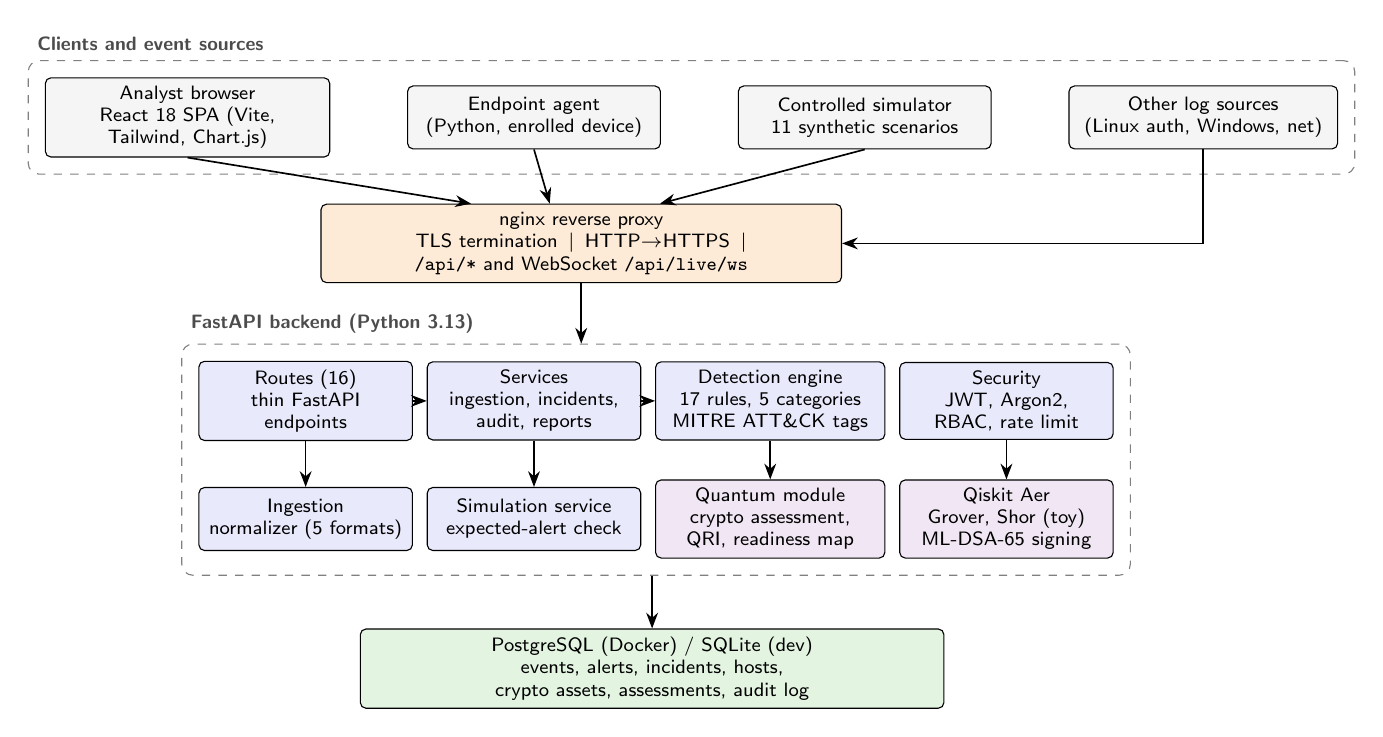
\begin{tikzpicture}[
  font=\sffamily\scriptsize,
  box/.style={draw, rounded corners=2pt, align=center, minimum height=8mm, inner sep=3pt},
  arr/.style={-{Stealth[length=2mm]}, semithick},
  grp/.style={draw, dashed, rounded corners=4pt, gray, inner sep=6pt}
]
% clients
\node[box, fill=gray!8, text width=3.4cm] (browser) at (0,0) {Analyst browser\\React 18 SPA (Vite, Tailwind, Chart.js)};
\node[box, fill=gray!8, text width=3.0cm] (agent)   at (4.4,0) {Endpoint agent\\(Python, enrolled device)};
\node[box, fill=gray!8, text width=3.0cm] (sim)     at (8.6,0) {Controlled simulator\\11 synthetic scenarios};
\node[box, fill=gray!8, text width=3.2cm] (other)   at (12.9,0) {Other log sources\\(Linux auth, Windows, net)};
\begin{scope}[on background layer]
\node[grp, fit=(browser)(agent)(sim)(other), label={[anchor=south west, font=\sffamily\scriptsize\bfseries, text=black!70]north west:Clients and event sources}] (cg) {};
\end{scope}
% proxy
\node[box, fill=proxy, text width=6.4cm] (nginx) at (5.0,-1.6) {nginx reverse proxy\\TLS termination \,$|$\, HTTP$\to$HTTPS \,$|$\, \texttt{/api/*} and WebSocket \texttt{/api/live/ws}};
\draw[arr] (browser.south) -- (nginx.north -| 3.6,0);
\draw[arr] (agent.south) -- (nginx.north -| 4.6,0);
\draw[arr] (sim.south) -- (nginx.north -| 6.0,0);
\draw[arr] (other.south) |- (nginx.east);
% backend
\node[box, fill=siem,  text width=2.5cm] (routes) at (1.5,-3.6) {Routes (16)\\thin FastAPI endpoints};
\node[box, fill=siem,  text width=2.5cm] (serv)   at (4.4,-3.6) {Services\\ingestion, incidents, audit, reports};
\node[box, fill=siem,  text width=2.7cm] (det)    at (7.4,-3.6) {Detection engine\\17 rules, 5 categories\\MITRE ATT\&CK tags};
\node[box, fill=siem,  text width=2.5cm] (sec)    at (10.4,-3.6) {Security\\JWT, Argon2, RBAC, rate limit};
\node[box, fill=siem,  text width=2.5cm] (ing)    at (1.5,-5.1) {Ingestion\\normalizer (5 formats)};
\node[box, fill=siem,  text width=2.5cm] (simsv)  at (4.4,-5.1) {Simulation service\\expected-alert check};
\node[box, fill=quant, text width=2.7cm] (qmod)   at (7.4,-5.1) {Quantum module\\crypto assessment, QRI, readiness map};
\node[box, fill=quant, text width=2.5cm] (qisk)   at (10.4,-5.1) {Qiskit Aer\\Grover, Shor (toy)\\ML-DSA-65 signing};
\draw[arr] (routes) -- (serv); \draw[arr] (serv) -- (det);
\draw[arr] (routes) -- (ing); \draw[arr] (serv) -- (simsv); \draw[arr] (det) -- (qmod); \draw[arr] (sec) -- (qisk);
\begin{scope}[on background layer]
\node[grp, fit=(routes)(sec)(ing)(qisk), label={[anchor=south west, font=\sffamily\scriptsize\bfseries, text=black!70]north west:FastAPI backend (Python 3.13)}] (bg) {};
\end{scope}
\draw[arr] (nginx.south) -- (nginx.south |- bg.north);
% persistence
\node[box, fill=persist, text width=7.2cm] (db) at (5.9,-7.0) {PostgreSQL (Docker) / SQLite (dev)\\events, alerts, incidents, hosts, crypto assets, assessments, audit log};
\draw[arr] (bg.south -| db.north) -- (db.north);
\end{tikzpicture}
\caption{Q-SOC system architecture as implemented. Blue: SIEM/SOC components; violet: quantum components; green: persistence.}
\label{fig:arch}
\end{figure*}

% ---------------- Fig. 2: data pipelines ----------------
\begin{figure*}[t]
\centering
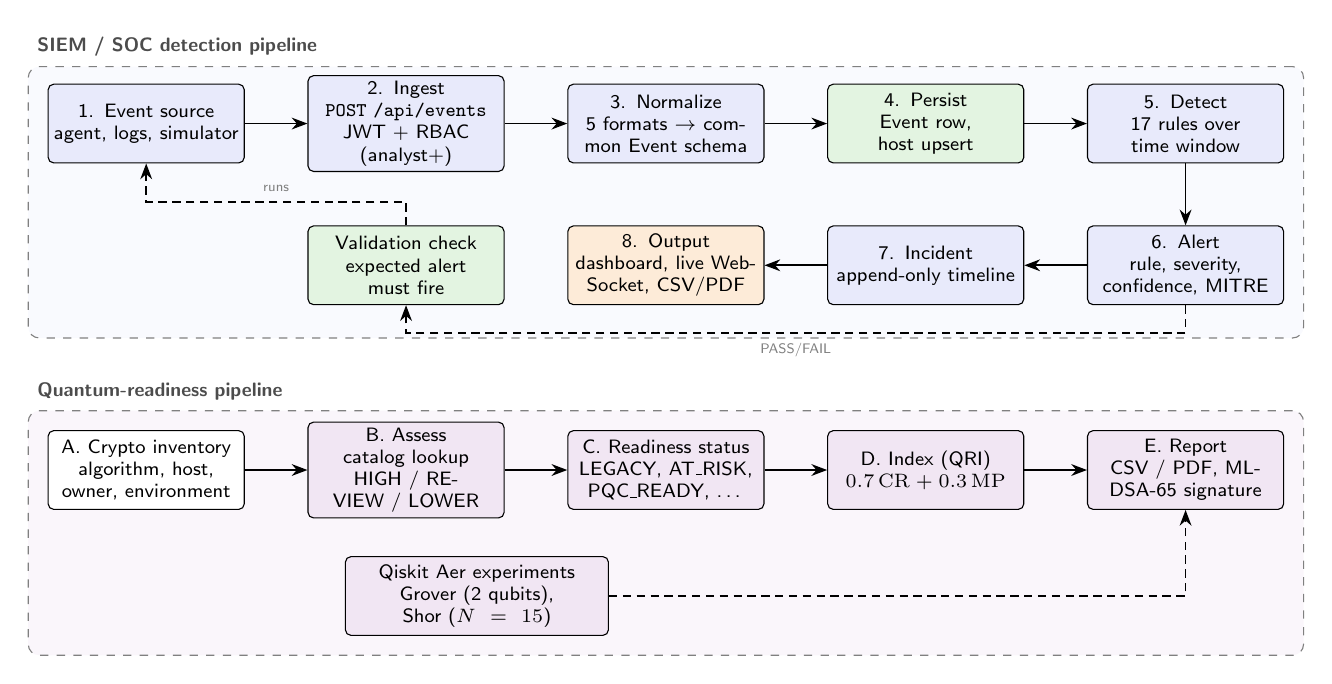
\begin{tikzpicture}[
  font=\sffamily\scriptsize,
  st/.style={draw, rounded corners=2pt, align=center, text width=2.35cm, minimum height=10mm, inner sep=2pt},
  arr/.style={-{Stealth[length=2mm]}, semithick},
  darr/.style={-{Stealth[length=2mm]}, semithick, densely dashed},
  grp/.style={draw, dashed, rounded corners=4pt, gray, inner sep=7pt}
]
% detection row 1
\node[st, fill=siem] (s1) at (0,0)     {1. Event source\\agent, logs, simulator};
\node[st, fill=siem] (s2) at (3.3,0)   {2. Ingest\\\texttt{POST /api/events}\\JWT + RBAC (analyst+)};
\node[st, fill=siem] (s3) at (6.6,0)   {3. Normalize\\5 formats $\to$ common Event schema};
\node[st, fill=persist] (s4) at (9.9,0){4. Persist\\Event row, host upsert};
\node[st, fill=siem] (s5) at (13.2,0)  {5. Detect\\17 rules over time window};
% row 2
\node[st, fill=siem] (s6) at (13.2,-1.8) {6. Alert\\rule, severity, confidence, MITRE};
\node[st, fill=siem] (s7) at (9.9,-1.8)  {7. Incident\\append-only timeline};
\node[st, fill=proxy] (s8) at (6.6,-1.8) {8. Output\\dashboard, live WebSocket, CSV/PDF};
\node[st, fill=persist] (val) at (3.3,-1.8) {Validation check\\expected alert must fire};
\draw[arr] (s1)--(s2); \draw[arr] (s2)--(s3); \draw[arr] (s3)--(s4); \draw[arr] (s4)--(s5);
\draw[arr] (s5)--(s6); \draw[arr] (s6)--(s7); \draw[arr] (s7)--(s8);
\draw[darr] (s6.south) -- ++(0,-0.35) -| node[pos=0.25, below, font=\sffamily\tiny, gray]{PASS/FAIL} (val.south);
\draw[darr] (val.north) -- ++(0,0.3) -| node[pos=0.25, above, font=\sffamily\tiny, gray]{runs} (s1.south);
\begin{scope}[on background layer]
\node[grp, fill=siem!25, fit=(s1)(s5)(s6)(val), yshift=-1mm, inner ysep=9pt, label={[anchor=south west, font=\sffamily\scriptsize\bfseries, text=black!70]north west:SIEM / SOC detection pipeline}] {};
\end{scope}
% quantum row
\node[st, fill=white] (qa) at (0,-4.4)   {A. Crypto inventory\\algorithm, host, owner, environment};
\node[st, fill=quant] (qb) at (3.3,-4.4) {B. Assess\\catalog lookup\\HIGH / REVIEW / LOWER};
\node[st, fill=quant] (qc) at (6.6,-4.4) {C. Readiness status\\LEGACY, AT\_RISK, PQC\_READY, \ldots};
\node[st, fill=quant] (qd) at (9.9,-4.4) {D. Index (QRI)\\$0.7\,\mathrm{CR}+0.3\,\mathrm{MP}$};
\node[st, fill=quant] (qe) at (13.2,-4.4){E. Report\\CSV / PDF, ML-DSA-65 signature};
\node[st, fill=quant, text width=3.2cm] (qk) at (4.2,-6.0) {Qiskit Aer experiments\\Grover (2 qubits), Shor ($N=15$)};
\draw[arr] (qa)--(qb); \draw[arr] (qb)--(qc); \draw[arr] (qc)--(qd); \draw[arr] (qd)--(qe);
\draw[darr] (qk.east) -| (qe.south);
\begin{scope}[on background layer]
\node[grp, fill=quant!35, fit=(qa)(qe)(qk), label={[anchor=south west, font=\sffamily\scriptsize\bfseries, text=black!70]north west:Quantum-readiness pipeline}] {};
\end{scope}
\end{tikzpicture}
\caption{Data pipelines. Top: ingestion, detection, alerting and incident handling, with the validation check that confirms a simulated scenario produced its expected alert. Bottom: cryptographic inventory to Quantum Readiness Index and signed report.}
\label{fig:pipeline}
\end{figure*}

\subsection{Detection data pipeline}
Fig.~\ref{fig:pipeline} is, for all practical purposes, following any event from its origin to the analyst. (1)~The source is sending a raw payload to \code{/api/events} or \code{/api/events/batch} in one of five formats (generic, Linux auth, Windows Security, network, simulator); only the analyst and admin roles may, in effect, write. (2)~The normalizer translates the payload into one typical Event schema (timestamp, host, event type, severity, user, tackles, message, raw event). (3)~The event is stored and its host record is modified. (4)~The Every rule module is performed by detection engine, and each person module retrieves its own time window from the database, so detections take previous events into the account together with the current batch. (5)~A further firing rule that is, broadly speaking, not a recent copy creates an Alert including rule, severity, confidence, evidence event identifiers and a MITRE ATT\&CK tag. Building on this observation, alerts are, in essence, acknowledged by (6)~Analysts and create Incidents that link alerts as indication; each note and status update is recorded as an append-only timeline entry. (7)~The dashboard, live stream and CSV/PDF reports are reading from the same tables. Detection is running synchronously within the ingest request.

\subsection{Verification of detection and the simulator}
Synthetic events with labels are created by the simulator (documentation-range tackles, 203.0.113.0/24) for 11 scenarios and is logging the related rule, severity, and MITRE tag that each should generate. A run is \emph{passing} solely if a new alert references that run's events and all three characteristics align; It is counted as a failure, if not; indeed, a mode called ``authorised lab'' does not inject anything and assesses actual telemetry from a permitted, registered endpoint. Out of 17 rules, just 4 have a direct ATT\&CK mapping; the code marks 7 as indicative and 6 as unmapped, meaning ATT\&CK labels shouldn't be construed as claims of coverage.

\subsection{Quantum-readiness pipeline}
Cryptographic assets (algorithm, framework, host, protocol, environment, owner) are, in this context, grouped as stated by a 21-entry catalog into HIGH (public-key strategies compromised by Shor's algorithm), REVIEW, and LOWER (symmetric and hash primitives influenced by Grover's algorithm at a reduced margin). Any autonomous mapping is creating a readiness status (LEGACY, AT\_RISK, PARTIALLY\_READY, PQC\_READY, UNKNOWN) grounded in the category and migration status. In light of this dynamic, crypto readiness (CR) is integrated by the QRI, migration preparedness (MP), and quantum exposure (QE) with experimental default weights of 0.4/0.3/0.3, signified in the interface as the proposed research metric. Given that CR and QE align in catalog-only inventories, $\mathrm{QRI}=0.7\,\mathrm{CR}+0.3\,\mathrm{MP}$ in that setting (verified accurately, Section~\ref{sec:results}). The Qiskit A 2-qubit space and factor $N$ are studied by examples $=15$ applying one more local Aer simulator; educational purposes are, in effect, served by them and are frequently not intended as attacks. The \code{cryptography} library is applied to sign reports with ML-DSA-65 (FIPS 204); hybrid TLS in nginx, post-quantum server certificates, and ML-DSA-signed JWTs are, in essence, marked as blocked or not realized in the repository's own status.

\subsection{Data model}
Storage is, in practice, handled via Alembic (three revisions, beginning with the quantum-only foundation and encompassing the SIEM/SOC and RBAC layer). Viewed through this lens, Table~\ref{tab:datamodel} is summarizing the 14 tables in the database reference; 15 ORM models are, put simply, stated by the code and also encompasses alert notes, indicators of compromise, and enrolled endpoints. Two design options are, in essence, prominent. First alerts save the identifiers of their evidence events, allowing each individual alert to be linked back to the original payload that triggered it. Second, one plaintext password is spanned by no column, secret, or token: an Argon2 hash is only kept by users, and secrets are reliably stored solely in environment variables. The development During the start-up, tables are yielded by route; while the PostgreSQL route rests on \code{alembic upgrade head}.

\begin{table*}[t]
\caption{Relational data model (from the migration scripts and ORM models).}
\label{tab:datamodel}
\centering
\footnotesize
\begin{tabularx}{\textwidth}{@{}l l X@{}}
\toprule
Table & Purpose & Principal columns and relations \\
\midrule
\code{users} & Accounts and roles & email (unique), Argon2 hash, role (admin/analyst/viewer), active flag \\
\code{events} & Normalized SIEM events & timestamp, source, host, event type, severity, user, source/destination address, port, message, raw JSON; indexed on seven columns \\
\code{detection\_rules} & Rule metadata & rule identifier (unique), category, severity, MITRE technique, enabled flag \\
\code{alerts} & Rule firings & rule, severity, confidence, status (OPEN/ACKNOWLEDGED/CLOSED), evidence event IDs, host, source address, acknowledging user \\
\code{incidents} & Investigations & title, status (six values), severity, assigned analyst, resolution, timestamps \\
\code{incident\_alerts} & Incident--alert links & foreign keys to incidents and alerts \\
\code{incident\_timeline} & Append-only trail & entry type (note, status change, alert linked), author, content, time \\
\code{hosts} & Asset directory & hostname, address, environment, owner, first/last seen; upserted on ingest \\
\code{audit\_logs} & Security-relevant actions & actor, action, target, JSON detail, time \\
\code{simulation\_runs} & Simulator history & scenario, triggering user, events generated, expected rule, detection confirmed \\
\code{crypto\_assets} & Cryptographic inventory & algorithm, system, purpose, key size, service, host, port, protocol, certificate info, environment, owner, readiness status \\
\code{quantum\_assessments} & Assessment results & optional asset link, crypto type, threat, risk class, migration status, recommendation, readiness status \\
\code{quantum\_experiments} & Qiskit runs & algorithm, backend, qubits, shots, duration, measurement counts, dominant result \\
\code{readiness\_scores} & QRI snapshots & component scores, weights, index, label \\
\bottomrule
\end{tabularx}
\end{table*}

\subsection{Security model}
The ingestion API is, in this setting, the one place where untrusted data enters, and the simulator is the one element that could be mistaken for offensive tooling, so both are curbed. Table~\ref{tab:rbac} gives the role model; Table~\ref{tab:controls} is, as it stands, listing the controls we found in the code and documentation. A viewer token that reaches a mutating endpoint receives HTTP 403 and not a degraded response; this is covered by tests for events, alerts, incidents and the simulator. Login is substantially limited to ten attempts per minute per client address applying an in-memory, per-process limiter; this is satisfactory for a person worker, but would not be shared across the workers.

\begin{table}[t]
\caption{Role-based access control.}
\label{tab:rbac}
\centering
\footnotesize
\begin{tabular}{@{}l c c c@{}}
\toprule
Role & Read & Ingest / simulate / manage & Users \\
\midrule
viewer  & yes & no  & no \\
analyst & yes & yes & no \\
admin   & yes & yes & future \\
\bottomrule
\end{tabular}
\end{table}

\begin{table}[t]
\caption{Security controls and the threat each addresses.}
\label{tab:controls}
\centering
\footnotesize
\begin{tabular}{@{}p{4.3cm} p{3.6cm}@{}}
\toprule
Control & Threat addressed \\
\midrule
JWT (HS256), secret from environment & Unauthenticated access; secrets in source \\
Argon2 password hashing & Credential disclosure from the database \\
Login rate limit, 10 per minute & Credential stuffing against the dashboard \\
Fixed ingestion formats, 400 on malformed & Unrecognized or partial payloads stored \\
ORM-only queries, Pydantic bodies & SQL injection \\
Audit log of logins, alert and incident changes, runs & Unaccountable privileged actions \\
Simulator posts only to its own API & Real attack traffic from a teaching tool \\
Documentation-range addresses (203.0.113.0/24) & Confusion with real hosts \\
Configurable CORS origins & Open cross-origin access \\
\bottomrule
\end{tabular}
\end{table}

\subsection{Application programming interface}
The backend exposes 16 route modules (admin, agent, alerts, auth, dashboard, endpoints, events, exports, incidents, IOCs, live, PQC, quantum, reports, rules, simulator). Table~\ref{tab:api} lists the principal endpoints that the evaluation touches. Deviations use a uniform \code{\{"detail": ...\}} body with 400 for malformed ingestion, 401 for authentication failures, 403 for part failures, 404 for missing resources, 422 for schema validation, 429 for login throttling and 500 for unhandled discrepancies. The frontend has 21 pages; an endpoint agent (about 600 non-blank lines) enrolls with a single-use token, buffers events while offline and is, in effect, rejected promptly after revocation, which the root test suite checks against a real server.

\begin{table}[t]
\caption{Principal API endpoints (A+: analyst or admin).}
\label{tab:api}
\centering
\scriptsize
\setlength{\tabcolsep}{3pt}
\begin{tabular}{@{}l l c p{2.2cm}@{}}
\toprule
Method & Path & Auth & Function \\
\midrule
POST  & \code{/api/auth/login} & none & Issue token \\
POST  & \code{/api/events[/batch]} & A+ & Normalize, store, detect \\
GET   & \code{/api/events} & any & Filtered event list \\
PATCH & \code{/api/alerts/\{id\}} & A+ & Acknowledge or close \\
POST  & \code{/api/incidents} & A+ & Open incident from alerts \\
GET   & \code{/api/dashboard/summary} & any & Combined KPIs \\
POST  & \code{/api/simulator/run} & A+ & Run a scenario \\
POST  & \code{/api/quantum/assess} & A+ & Classify an algorithm \\
GET   & \code{/api/quantum/readiness} & A+ & Compute and store QRI \\
GET   & \code{/api/quantum/grover|shor} & A+ & Run Qiskit demo \\
GET   & \code{/api/reports/readiness/pdf} & any & Signed readiness report \\
\bottomrule
\end{tabular}
\end{table}

% =====================================================================
\section{Detection Engine and Rule Catalogue}
% =====================================================================
\subsection{Event normalization}
Whatever the source, an event is reduced to one schema: timestamp, source, host, event type, severity, user, source address, destination address and port, message and the original payload. Table~\ref{tab:formats} lists the five accepted formats. Unknown formats, missing required fields and invalid severities, actions or Windows event identifiers raise a normalization error that is returned as HTTP 400, so nothing is partially stored. The Windows mapping covers only a documented subset of Security event identifiers and is not a claim of full Event Log coverage. The simulator format is normalized identically to the generic one, so detection rules never special-case simulated events; this is what allows the simulator to test the real path.

\begin{table}[t]
\caption{Accepted ingestion formats.}
\label{tab:formats}
\centering
\footnotesize
\setlength{\tabcolsep}{3pt}
\begin{tabular}{@{}l p{1.8cm} p{3.6cm}@{}}
\toprule
Format & Required fields & Mapping \\
\midrule
generic & host, event type & Pass-through; severity defaults to medium, time to now \\
linux\_auth & host, action & failed/invalid/accepted password or key, sudo, session $\to$ event type and severity \\
windows\_security & Computer, EventID & 4625, 4624, 4672, 4720, 4732 $\to$ failure, success, privilege use, account created, escalation \\
network & host, source address & Default type connection attempt; carries destination and protocol \\
simulator & as generic & Identical to generic \\
\bottomrule
\end{tabular}
\end{table}

\subsection{Rule catalogue}
17 rules in five modules (authentica- are encompassed by the engine tion, network, web and endpoint, with any second center on threat intelligence). Each module exports static metadata and the \code{evaluate} function, and all modules on every ingested batch are run by the engine, seeds the rule table idempotently, and suppresses alerts that are repeating Within five minutes, the same rule and host or source tackle. Table~\ref{tab:rules} lists every rule with its trigger, severity and ATT\&CK method as recorded in the code. Rules fall into two kinds: \emph{threshold} rules are specifically counting events per source address or host in a sliding window, and \emph{typed-event} rules fire when an event already carries a particular type. Threshold rules are, in essence, the ones with behaviour worth testing at their boundaries (Section~\ref{sec:results}); typed-event rules rely on the upstream producer, here the simulator or agent, to classify the event.

\begin{table*}[t]
\caption{Detection rule catalogue (17 rules). Triggers are from the detection-rule reference and were checked at their boundaries (E3); the technique column is the mapping in the code, with its quality (D: direct, I: indicative, --: none).}
\label{tab:rules}
\centering
\footnotesize
\begin{tabular}{@{}l l l l c@{}}
\toprule
Rule & Severity & Trigger & Technique & Q \\
\midrule
auth.repeated\_failed\_logins & medium & $\geq 5$ authentication failures, same source address, within 10 min & T1110 & D \\
auth.brute\_force\_burst & high & $\geq 10$ authentication failures, same source address, within 5 min & T1110 & D \\
auth.successful\_login\_after\_failures & high & Success preceded by $\geq 3$ failures from the same address within 10 min & T1078 & I \\
auth.privilege\_related\_activity & medium & Any privilege-use event (high if privilege escalation) & T1078 & I \\
network.repeated\_connection\_attempts & medium & $\geq 20$ connection attempts, same source, within 5 min & -- & -- \\
network.synthetic\_port\_scan & high & Connection attempts to $\geq 8$ distinct ports from one source within 2 min & T1046 & D \\
network.unexpected\_service\_access & medium & Event typed unexpected service access & -- & -- \\
web.repeated\_api\_auth\_failures & medium & $\geq 5$ API authentication failures, same source, within 5 min & T1110 & D \\
web.abnormal\_request\_rate & medium & $\geq 50$ API requests, same source, within 1 min & T1499 & I \\
web.suspicious\_request\_pattern & high & Event typed suspicious web request & T1190 & I \\
endpoint.suspicious\_process & medium & Event typed suspicious process & -- & -- \\
endpoint.privilege\_escalation\_indicator & high & Event typed privilege-escalation indicator & -- & -- \\
endpoint.persistence\_indicator & high & Event typed persistence indicator & T1547 & I \\
endpoint.suspicious\_file\_activity & medium & Single event typed suspicious file activity & -- & -- \\
endpoint.ransomware\_like\_file\_activity\_burst & critical & $\geq 5$ suspicious file-activity events, same host, within 2 min & T1486 & I \\
endpoint.data\_access\_anomaly & medium & Event typed data-access anomaly & T1005 & I \\
threat\_intel.ioc\_match & medium & Event field matches a stored (test) indicator & -- & -- \\
\bottomrule
\end{tabular}
\end{table*}

\subsection{Attack simulator}
Descriptive telemetry is only generated by the simulator. Its scenarios call the application's own ingestion path; they never open one socket to one more host, never issue a request to a third party and never run an operating-system tool. The port-scan scenario posts network events shaped like a scan, and the ransomware-like situation posts file-activity events outlining a mass rename, without yielding, renaming or encrypting any file. Running a case needs an analyst token, creates a simulation record and writes an audit entry. Table~\ref{tab:scenarios} recapitulates the 11 situations, one per projected rule family. The returned \code{detection\_confirmed} flag is the signal of interest, including it is true only if the declared rule actually raised an alert for that run. The situation for the threat-intelligence rule applies a manifestly labelled test indicator, and the brute-force scenario is marked as a lab procedure.

\begin{table}[t]
\caption{Simulator scenarios and generated events.}
\label{tab:scenarios}
\centering
\footnotesize
\begin{tabular}{@{}l r l@{}}
\toprule
Scenario & Events & Expected rule \\
\midrule
auth failure burst & 12 & brute\_force\_burst \\
repeated login attempts & 6 & repeated\_failed\_logins \\
success after failures & 5 & successful\_login\_after\_failures \\
synthetic port scan & 12 & synthetic\_port\_scan \\
suspicious web request & 1 & suspicious\_request\_pattern \\
privilege escalation & 1 & privilege\_escalation\_indicator \\
suspicious process & 1 & suspicious\_process \\
persistence indicator & 1 & persistence\_indicator \\
data access anomaly & 1 & data\_access\_anomaly \\
ransomware-like activity & 6 & ransomware\_like\_file\_burst \\
test indicator match & 1 & ioc\_match \\
\bottomrule
\end{tabular}
\end{table}

\subsection{Assessment catalog}
21 normalized algorithm is held by the quantum layer's catalog identifiers, namely seven HIGH, two REVIEW and twelve LOWER. Table~\ref{tab:catalog} is listing them. Each entry carries a type, a category, a migration status and a reference string that is always either a theoretical citation or a NIST document; the engine returns an unambiguous UNKNOWN for anything absent, in preference to a invented answer. In this broader context, the catalog is predominantly hand-curated and is uniformly not an formal NIST security-level assignment or a certified audit result.

\begin{table*}[t]
\caption{Assessment catalog (21 entries).}
\label{tab:catalog}
\centering
\footnotesize
\begin{tabular}{@{}l l l l l@{}}
\toprule
Algorithm & Purpose & Risk & Readiness & Basis \\
\midrule
RSA-2048 / 3072 / 4096 & key establishment & HIGH & LEGACY & Shor; NIST PQC guidance \\
ECDH, DH-2048 & key establishment & HIGH & LEGACY & Shor; NIST IR 8547 draft transition plan \\
ECDSA, ECC & signature & HIGH & LEGACY & Shor (extended to elliptic curves) \\
AES-128 & symmetric & REVIEW & AT\_RISK & Grover; reduced strength margin \\
SHA-256 & hash & REVIEW & AT\_RISK & Grover; reduced preimage margin \\
AES-256, HMAC-SHA256 & symmetric / MAC & LOWER & PARTIALLY\_READY & Grover; adequate margin \\
SHA-384, Argon2id & hash / KDF & LOWER & PARTIALLY\_READY & Grover; RFC 9106 for Argon2id \\
ML-KEM-512 / 768 / 1024 & key establishment & LOWER & PQC\_READY & NIST FIPS 203 \\
ML-DSA-44 / 65 / 87 & signature & LOWER & PQC\_READY & NIST FIPS 204 \\
SLH-DSA & signature & LOWER & PQC\_READY & NIST FIPS 205 \\
X25519MLKEM768 & hybrid key exchange & LOWER & PQC\_READY & FIPS 203 component; IETF hybrid draft \\
\bottomrule
\end{tabular}
\end{table*}

\subsection{What Q-SOC itself employs}
The store classifies its own cryptography, which is a valuable consistency check for a readiness tool. Report and export signatures apply ML-DSA-65 with a context string, and the round trip is tested. Argon2id are employed by passwords, and session tokens apply an HMAC-SHA256 JWT, which is a symmetric construction outside Shor's reach but not a post-quantum signature. Under these conditions, the lab TLS certificate uses RSA-3072 and is therefore reported as LEGACY, because post-quantum certificates are not yet broadly supported by browsers, agents or certificate authorities. The hybrid X25519MLKEM768 key exchange in nginx was showed by a handshake test against a local server, but the nginx and Docker side was not executed in the build environment. Because, the RSA certificate stays flagged, the platform is deliberately not reported as fully quantum ready and its own index remains below 100.

% =====================================================================
\section{Demonstration Run and Interface Outputs}\label{sec:demo}
% =====================================================================
To reveal what an analyst sees without counting on interface images, this section reports the contents of the application's dashboard, alert, validation, inventory, readiness and experiment pages as tables and graphs, created by script from the application's own API (\code{scripts/make\_demo\_figs.py}, data in \code{data/demo\_data.json}). The instance was a development-mode rollout (FastAPI with SQLite, Vite-served frontend), populated only through the application's own interfaces, namely the 11 simulator scenarios were run, one incident was opened from three of the consequent alerts, ten cryptographic assets were added to the two seeded ones and assessed, and the Grover and Shor trials were, in practice, executed. All data are synthetic and all tackles are widely in the documentation range.

\textbf{Dashboard.} Table~\ref{tab:dashboard} is listing the indicators this dashboard shows after the run. Fig.~\ref{fig:demo} is distributing the 11 alerts by severity and rule category and the events per host. Validation was passed by all 11 cases and none failed, and the one critical alert came from the ransomware-like file-activity scenario.

\begin{table}[t]
\caption{Dashboard indicators after the demonstration run.}
\label{tab:dashboard}
\centering
\footnotesize
\begin{tabular}{@{}l r@{}}
\toprule
Indicator & Value \\
\midrule
Total events & 47 \\
Alerts (critical / high / medium) & 11 (1 / 6 / 4) \\
Active incidents & 1 \\
Validation runs passed / failed & 11 / 0 \\
Threat-intel indicators (active / test) & 5 / 5 \\
Threat-intel matches & 1 \\
Crypto inventory assets / assessments & 12 / 10 \\
Quantum-vulnerable algorithms (assessed) & 4 \\
Quantum Readiness Index & 54 \\
Migration readiness & 40.0\% \\
Qiskit experiments run & 2 \\
\bottomrule
\end{tabular}
\end{table}

% ---------------- Fig. 3 ----------------
\begin{figure*}[t]
\centering
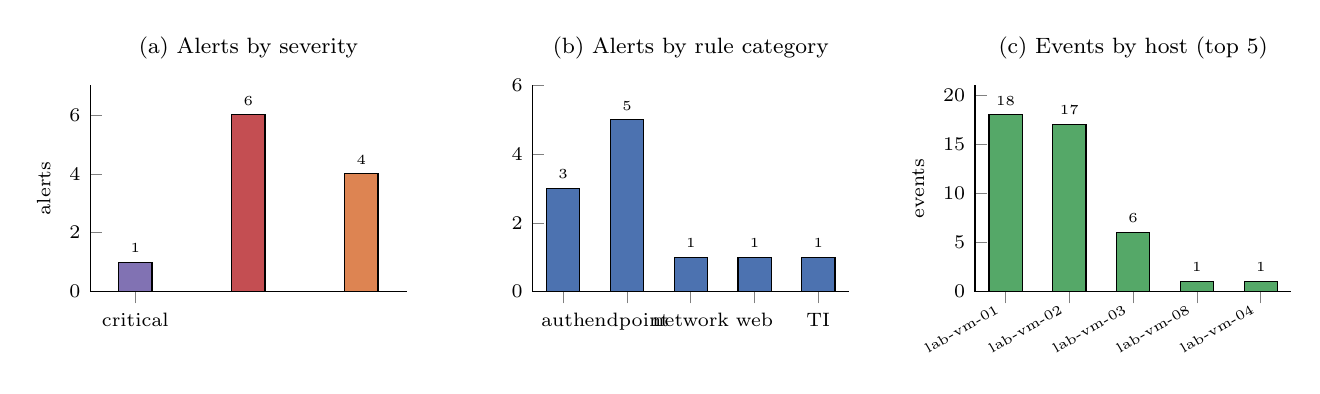
\begin{tikzpicture}
\begin{groupplot}[
  group style={group size=3 by 1, horizontal sep=1.6cm},
  width=5.6cm, height=4.2cm, ybar, /pgf/bar width=12pt,
  ymin=0, enlarge x limits=0.2, axis x line*=bottom, axis y line*=left,
  nodes near coords, every node near coord/.append style={font=\tiny},
  tick label style={font=\scriptsize}, title style={font=\footnotesize},
  label style={font=\scriptsize}
]
\nextgroupplot[title={(a) Alerts by severity}, ylabel={alerts},
  symbolic x coords={critical,high,medium}, xtick=data, ymax=7, bar shift=0pt]
\addplot[fill=cpurple, draw=black] coordinates {(critical,1)};
\addplot[fill=cred,    draw=black] coordinates {(high,6)};
\addplot[fill=corange, draw=black] coordinates {(medium,4)};
\nextgroupplot[title={(b) Alerts by rule category},
  symbolic x coords={auth,endpoint,network,web,TI}, xtick=data, ymax=6, enlarge x limits=0.12]
\addplot[fill=cblue, draw=black] coordinates {(auth,3) (endpoint,5) (network,1) (web,1) (TI,1)};
\nextgroupplot[title={(c) Events by host (top 5)}, ylabel={events},
  % NOTE: host names were unreadable in the source; edit to match data/demo_data.json
  symbolic x coords={lab-vm-01,lab-vm-02,lab-vm-03,lab-vm-08,lab-vm-04}, xtick=data,
  ymax=21, enlarge x limits=0.12, x tick label style={rotate=30, anchor=east, font=\tiny}]
\addplot[fill=cgreen, draw=black] coordinates {(lab-vm-01,18) (lab-vm-02,17) (lab-vm-03,6) (lab-vm-08,1) (lab-vm-04,1)};
\end{groupplot}
\end{tikzpicture}
\caption{Demonstration run (47 events, 11 alerts): (a) alerts by severity, (b) alerts by detection-rule category (TI: threat intelligence), (c) events by host.}
\label{fig:demo}
\end{figure*}

\textbf{Alerts and detection validation.} Table~\ref{tab:demoalerts} lays out, for each individual simulator scenario, the rule it is predominantly anticipated to trigger, the projected severity and ATT\&CK technique, the confidence of the ensuing alert, the number of events the situation produced and the outcome. The outcome column is typically obtained by checking the alert raised by the application with the scenario's declared expectation; it is agreeing with the application's own validation tally of 11 passed and 0 failed. Three scenarios (privilege escalation, suspicious process and the threat-No ATT\&CK technique tag is had in this by intelligence match) run. Alerts are starting as open and the analyst can admit them or link them to one more incident, which in this run carried any timeline of the creation note, the status are changing to STUDYING and one analyst note.

\begin{table*}[t]
\caption{Simulator scenarios, expected detections and observed alerts in the demonstration run (events sum to 47).}
\label{tab:demoalerts}
\centering
\footnotesize
\begin{tabular}{@{}l l l c c r c@{}}
\toprule
Scenario & Expected rule & Severity & Conf. & ATT\&CK & Events & Result \\
\midrule
auth\_failure\_burst & \code{auth.brute\_force\_burst} & high & 0.85 & T1110 & 12 & PASS \\
repeated\_login\_attempts & \code{auth.repeated\_failed\_logins} & medium & 0.70 & T1110 & 6 & PASS \\
successful\_login\_after\_failures & \code{auth.successful\_login\_after\_failures} & high & 0.80 & T1078 & 5 & PASS \\
synthetic\_port\_scan & \code{network.synthetic\_port\_scan} & high & 0.80 & T1046 & 12 & PASS \\
suspicious\_web\_request & \code{web.suspicious\_request\_pattern} & high & 0.75 & T1190 & 1 & PASS \\
privilege\_escalation\_indicator & \code{endpoint.privilege\_escalation\_indicator} & high & 0.80 & none & 1 & PASS \\
suspicious\_process\_event & \code{endpoint.suspicious\_process} & medium & 0.70 & none & 1 & PASS \\
persistence\_indicator & \code{endpoint.persistence\_indicator} & high & 0.80 & T1547 & 1 & PASS \\
data\_access\_anomaly & \code{endpoint.data\_access\_anomaly} & medium & 0.65 & T1005 & 1 & PASS \\
ransomware\_like\_file\_activity & \code{endpoint.ransomware\_like\_file\_activity\_burst} & critical & 0.90 & T1486 & 6 & PASS \\
ioc\_test\_indicator\_match & \code{threat\_intel.ioc\_match} & medium & 1.00 & none & 1 & PASS \\
\bottomrule
\end{tabular}
\end{table*}

\textbf{Quantum security pages.} Table~\ref{tab:demoinv} is listing the cryptographic inventory with the risk classification from the assessment engine and the formulated readiness status. Fig.~\ref{fig:qri} recapitulates the three QRI components, the readiness-status distribution of the 12 assets and the risk classification of the 10 assessments. With component scores of 60, 40 and 60 and the default weights, the index is $0.4\cdot 60 + 0.3\cdot 40 + 0.3\cdot 60 = 54$. Four assessed algorithms (RSA-2048, RSA-3072, ECDSA and ECDH) are classified HIGH risk, AES-128 and SHA-256 REVIEW, AES-256 and ML-DSA-65 LOWER, and 3DES and SHA-1 UNKNOWN because the catalog enters for them; Section~\ref{sec:results} is explaining why that last case matters for the index. Two seeded assets are, in essence, pointed to as not assessed.

\begin{table}[t]
\caption{Cryptographic inventory of the demonstration run.}
\label{tab:demoinv}
\centering
\footnotesize
\setlength{\tabcolsep}{3pt}
\begin{tabular}{@{}l l l l@{}}
\toprule
Algorithm & Host & Risk class & Readiness status \\
\midrule
ML-DSA-65 & q-soc & LOWER & PQC\_READY \\
3DES & pay-gw & UNKNOWN & UNKNOWN \\
SHA-1 & legacy-01 & UNKNOWN & UNKNOWN \\
SHA-256 & ci-01 & REVIEW & AT\_RISK \\
AES-128 & backup-01 & REVIEW & AT\_RISK \\
AES-256 & db-01 & LOWER & PARTIALLY\_READY \\
ECDH-P256 & web-01 & HIGH & LEGACY \\
RSA-3072 & vpn.example.internal & HIGH & LEGACY \\
ECDSA-P256 & build-01 & HIGH & LEGACY \\
RSA-2048 & api.example.internal & HIGH & LEGACY \\
AES-256 & seeded demo asset & not assessed & NOT\_ASSESSED \\
RSA-2048 & portal.lab.local & not assessed & NOT\_ASSESSED \\
\bottomrule
\end{tabular}
\end{table}

% ---------------- Fig. 4 ----------------
\begin{figure*}[t]
\centering
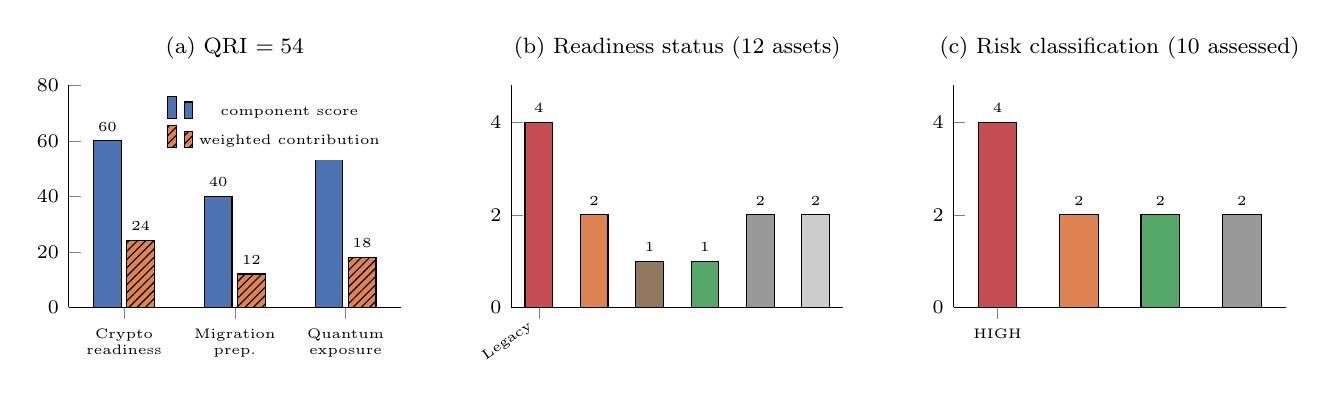
\begin{tikzpicture}
\begin{groupplot}[
  group style={group size=3 by 1, horizontal sep=1.4cm},
  width=5.8cm, height=4.4cm, ymin=0, axis x line*=bottom, axis y line*=left,
  tick label style={font=\scriptsize}, title style={font=\footnotesize},
  nodes near coords, every node near coord/.append style={font=\tiny}
]
\nextgroupplot[title={(a) QRI $=54$}, ybar, bar width=10pt, ymax=80,
  symbolic x coords={CR,MP,QE}, xtick=data, enlarge x limits=0.25,
  xticklabels={Crypto readiness, Migration prep., Quantum exposure},
  x tick label style={font=\tiny, align=center, text width=1.4cm},
  legend style={font=\tiny, at={(0.98,0.98)}, anchor=north east, draw=none}]
\addplot[fill=cblue, draw=black] coordinates {(CR,60) (MP,40) (QE,60)};
\addplot[fill=corange, draw=black, postaction={pattern=north east lines}] coordinates {(CR,24) (MP,12) (QE,18)};
\legend{component score, weighted contribution}
\nextgroupplot[title={(b) Readiness status (12 assets)}, ybar, bar width=10pt, ymax=4.8,
  symbolic x coords={Legacy,At risk,Partly ready,PQC ready,Unknown,Not assessed}, xtick=data,
  enlarge x limits=0.1, x tick label style={rotate=35, anchor=east, font=\tiny}, bar shift=0pt]
\addplot[fill=cred,    draw=black] coordinates {(Legacy,4)};
\addplot[fill=corange, draw=black] coordinates {(At risk,2)};
\addplot[fill=cbrown,  draw=black] coordinates {(Partly ready,1)};
\addplot[fill=cgreen,  draw=black] coordinates {(PQC ready,1)};
\addplot[fill=cgray,   draw=black] coordinates {(Unknown,2)};
\addplot[fill=clgray,  draw=black] coordinates {(Not assessed,2)};
\nextgroupplot[title={(c) Risk classification (10 assessed)}, ybar, bar width=14pt, ymax=4.8,
  symbolic x coords={HIGH,REVIEW,LOWER,UNKNOWN}, xtick=data, enlarge x limits=0.18,
  x tick label style={font=\tiny}, bar shift=0pt]
\addplot[fill=cred,    draw=black] coordinates {(HIGH,4)};
\addplot[fill=corange, draw=black] coordinates {(REVIEW,2)};
\addplot[fill=cgreen,  draw=black] coordinates {(LOWER,2)};
\addplot[fill=cgray,   draw=black] coordinates {(UNKNOWN,2)};
\end{groupplot}
\end{tikzpicture}
\caption{Quantum-readiness outputs of the demonstration run: (a) QRI component scores and weighted contributions (QRI\,=\,54), (b) readiness status of the 12 inventory assets, (c) risk classification of the 10 assessments.}
\label{fig:qri}
\end{figure*}

\textbf{Trials page.} Fig.~\ref{fig:qiskit} is revealing the measurement counts recorded by the two Qiskit experiments. The 2-qubit Grover The marked state \code{11} was returned in all 1024 shots on the by search noiseless simulator. The Shor demonstration for $N=15$, $a=7$ returned four roughly equiprobable outcomes (0, 4, 8, 12 of 16), coherent with an order $r=4$, from which $\gcd(7^2\pm 1, 15)$ gives the factors 3 and 5. Both are, in effect, toy instances on a standard simulator.

% ---------------- Fig. 5 ----------------
\begin{figure}[t]
\centering
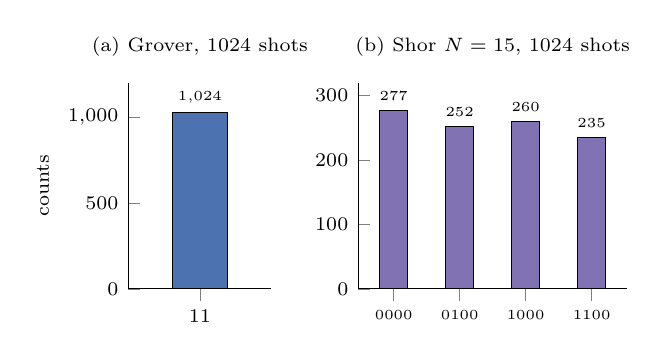
\begin{tikzpicture}
\begin{groupplot}[
  group style={group size=2 by 1, horizontal sep=1.1cm},
  height=4.2cm, ybar, ymin=0, axis x line*=bottom, axis y line*=left,
  tick label style={font=\scriptsize}, title style={font=\scriptsize},
  nodes near coords, every node near coord/.append style={font=\tiny}
]
\nextgroupplot[width=3.4cm, title={(a) Grover, 1024 shots}, ylabel={counts}, ylabel style={font=\scriptsize},
  symbolic x coords={11}, xtick=data, bar width=20pt, ymax=1200, enlarge x limits=0.6]
\addplot[fill=cblue, draw=black] coordinates {(11,1024)};
\nextgroupplot[width=5.0cm, title={(b) Shor $N=15$, 1024 shots},
  symbolic x coords={0000,0100,1000,1100}, xtick=data, bar width=10pt, ymax=320, enlarge x limits=0.18,
  x tick label style={font=\tiny}]
\addplot[fill=cpurple, draw=black] coordinates {(0000,277) (0100,252) (1000,260) (1100,235)};
\end{groupplot}
\end{tikzpicture}
\caption{Measurement counts recorded by the Qiskit experiments page (local Aer simulator).}
\label{fig:qiskit}
\end{figure}

% =====================================================================
\section{Evaluation Method}\label{sec:method}
% =====================================================================
All experiments import the unmodified backend and write raw CSV/JSON results, from which the figures and the signing table are generated. Host: Linux VM, 2 vCPU (i7-1255U), 3.9\,GB RAM, Python 3.13.16, Qiskit 2.5.2, Aer 0.17.2, SQLite; Docker, PostgreSQL and nginx were not used. Random seeds are recorded in the result files (QRI inventories: seed 20261013). Experiments (Table~\ref{tab:design}): R1 (QRI properties, 2000 random inventories of 3--30 assets), E1 (HTTP ingestion on a real uvicorn server, 11,800 events), E2 (scenario validation, 20 repetitions $\times$ 11 scenarios, fresh database each), E3 (24 boundary cases), E5 (shared-address noise, synthetic), E9 (37 malformed-input cases), Q1--Q3 (Qiskit) and S1 (signing cost, 30 repetitions).

Each experiment writes its raw rows to CSV or JSON together with the environment record (operating system, Python and package versions, repository commit d7ad437 and a flag stating that the working tree equalled HEAD), so the tables and figures can be regenerated without re-running the workload. Four design principles guided the harness. (i)~The system under test is the unmodified backend, imported or started as a server, so there is no re-implementation to drift from the product. (ii)~Every positive check has a negative control: the scenario validation is repeated with the expected rule disabled, which must fail. (iii)~Expectations are written from the documented specification before the run, and a deviation is reported as a finding rather than adjusted. (iv)~Synthetic parameters (for example the failure probability in E5) are stated, and results from them are described as properties of the thresholds, not as field measurements.

\begin{table*}[t]
\caption{Experiment design.}
\label{tab:design}
\centering
\footnotesize
\begin{tabularx}{\textwidth}{@{}l l X l l@{}}
\toprule
ID & Question & Workload & Metrics & Runs \\
\midrule
E1 & Throughput, latency & HTTP ingestion to a live uvicorn server; heartbeat, authentication success and failure events; batch size $B\in\{1,10,100,500\}$; read endpoints on 11,800 stored events & Events/s, request latency, alerts raised, read latency & 100/30/10/5 per $B$; 30 per read \\
E2 & Scenario validation & 11 scenarios, fresh database per run; same with the expected rule disabled; immediate re-run & Pass/fail, latency, severity match & $20\times 11 + 33 + 11$ \\
E3 & Rule boundaries & Event sequences at, just below and just above each threshold; window edges; evasion; deduplication & Fire/no-fire vs.\ specification & 24 cases \\
E5 & Shared-address noise & $U\in\{25,100,400,1000\}$ benign users behind one address, six attempts per day, failure probability $p\leq 0.10$ & Alerts per day by rule & 5 seeds per cell \\
E9 & Input robustness & 30 malformed or unusual payloads plus 7 protocol-level checks & HTTP status, server failure, conformance & 37 cases \\
R1 & QRI properties & Random inventories of 3--30 assets drawn with replacement from the catalog; 66 weight vectors & Equality of components, rank correlation & 2000 inventories \\
Q1--Q3 & Quantum demonstrations & Grover on 2 qubits, ideal and under depolarizing noise; Shor for $N=15$ & Success probability, depth, gate counts & 80 / 20 per noise level / 50 \\
S1 & Signing cost & ML-DSA-65, ECDSA P-256, RSA-3072-PSS; 1\,KiB to 10\,MiB & Sign and verify time, sizes & 30 \\
\bottomrule
\end{tabularx}
\end{table*}

% =====================================================================
\section{Results}\label{sec:results}
% =====================================================================
\subsection{Detection validation (E2, E3)}
All 220 simulator runs passed; with the anticipated rule disabled, 33 of 33 runs failed, so the check is sensitive to the rule rather than empty. In-process median latency was roughly 20--36\,ms (p95 30--71\,ms). Over HTTP on the loaded database all 11 situations still passed (52--73\,ms). The 24 boundary cases conformed to the rule specification. Three behaviours matter for users. In streaming mode \code{repeated\_failed\_logins} fires at event 5 and \code{brute\_force\_burst} at event 10, so Within any batch, ``supersedes'' is holding only. Ten failures spaced one hour apart (low-and-slow) and 20 failures from 20 sources (distributed) created no alert, the second by-design limit of tackle-keyed windows. Finally, six cases without one source address failed when re-run instantly inside the deduplication window; while the five with tackles passed.

Table~\ref{tab:perscenario} and Fig.~\ref{fig:latency} are giving the per-scenario view. Latency is, in this setting, mostly lowest for the single-event typed rules and higher for the multi-event threshold scenarios, as projected from the number of events normalized and queried. The immediate re-run column is separating the deduplication finding, namely the six situations that fail on a second run are those whose events carry no source address, so the suppression key can't distinguish the second run from the first. An analyst re-running such a situation would therefore see a failure that reflects the suppression policy, not a defect in the rule.

The boundary table (Table~\ref{tab:boundary}) is revealing that each individual threshold is executed as stipulated: the rule is, in effect, silent one event below the limit and fires exactly at it. The window cases are validating that the span, and not the count alone, is deciding, and the evasion rows are recording what the specification can't catch. Two further details are, in effect, worth stating. In cases B02 and B17 the higher rule and an alert for the was raised by its lower-threshold companion both same sequence, so two alerts exist for one behaviour; in B01 and B16 a lower-severity companion rule raised an alert when the higher rule did not, which is the intended escalation ladder.

\begin{table*}[t]
\caption{Per-scenario results (E2): 20 runs each, in-process latency in ms, negative control (rule disabled, 3 runs each) and immediate re-run inside the five-minute deduplication window.}
\label{tab:perscenario}
\centering
\footnotesize
\begin{tabular}{@{}l r r r r c c@{}}
\toprule
Scenario & Events & Median & p95 & Pass (of 20) & Control (rule off) & Immediate re-run \\
\midrule
auth\_failure\_burst & 12 & 36.2 & 51.0 & 20 & fail 3/3 & pass \\
repeated\_login\_attempts & 6 & 28.7 & 55.0 & 20 & fail 3/3 & pass \\
successful\_login\_after\_failures & 5 & 25.0 & 35.5 & 20 & fail 3/3 & pass \\
synthetic\_port\_scan & 12 & 31.6 & 43.6 & 20 & fail 3/3 & pass \\
suspicious\_web\_request & 1 & 20.2 & 30.4 & 20 & fail 3/3 & pass \\
privilege\_escalation\_indicator & 1 & 19.6 & 39.4 & 20 & fail 3/3 & \textbf{fail} \\
suspicious\_process\_event & 1 & 20.2 & 39.8 & 20 & fail 3/3 & \textbf{fail} \\
persistence\_indicator & 1 & 23.4 & 51.5 & 20 & fail 3/3 & \textbf{fail} \\
data\_access\_anomaly & 1 & 23.3 & 52.1 & 20 & fail 3/3 & \textbf{fail} \\
ransomware\_like\_file\_activity & 6 & 28.1 & 55.4 & 20 & fail 3/3 & \textbf{fail} \\
ioc\_test\_indicator\_match & 1 & 32.0 & 70.9 & 20 & fail 3/3 & \textbf{fail} \\
\bottomrule
\end{tabular}
\end{table*}

\begin{table*}[t]
\caption{Boundary, window, evasion and deduplication cases (E3). ``Fires'' is the observed outcome; all 24 cases conformed to the rule specification.}
\label{tab:boundary}
\centering
\footnotesize
\begin{tabular}{@{}l l l l l@{}}
\toprule
ID & Rule under test & Input & Expected & Fires \\
\midrule
B01/B02 & brute\_force\_burst & 9 / 10 failed logins, 1\,s apart & no / yes & no / yes (event 10) \\
B03/B04 & repeated\_failed\_logins & 4 / 5 failed logins, 10\,s apart & no / yes & no / yes (event 5) \\
B05/B06 & success\_after\_failures & 2 / 3 failures then a success, same source & no / yes & no / yes \\
B07/B08 & synthetic\_port\_scan & 7 / 8 distinct ports, 5\,s apart & no / yes & no / yes \\
B09 & synthetic\_port\_scan & 8 attempts to the same port & no & no \\
B10/B11 & repeated\_connection\_attempts & 19 / 20 attempts, same port & no / yes & no / yes \\
B12/B13 & repeated\_api\_auth\_failures & 4 / 5 API failures, 5\,s apart & no / yes & no / yes \\
B14/B15 & abnormal\_request\_rate & 49 / 50 requests in 60\,s & no / yes & no / yes \\
B16/B17 & ransomware\_like\_burst & 4 / 5 file events, one host, 10\,s apart & no / yes & no / yes \\
W01 & brute\_force\_burst & 10 failures, 40\,s apart (span 360\,s $>$ 300\,s) & no & no \\
W02 & repeated\_failed\_logins & same 10 failures, 600\,s window & yes & yes (event 5) \\
W03 & repeated\_failed\_logins & 5 failures, 160\,s apart (span 640\,s) & no & no \\
E01 & repeated\_failed\_logins & low-and-slow: 10 failures, 1\,h apart & (evasion) & no alert \\
E02/E03 & repeated\_failed / brute\_force & distributed: 20 failures from 20 sources & (evasion) & no alert \\
D01 & brute\_force\_burst & two 12-failure bursts, 2\,min apart & one alert & one alert \\
\bottomrule
\end{tabular}
\end{table*}

% ---------------- Fig. 6 ----------------
\begin{figure}[t]
\centering
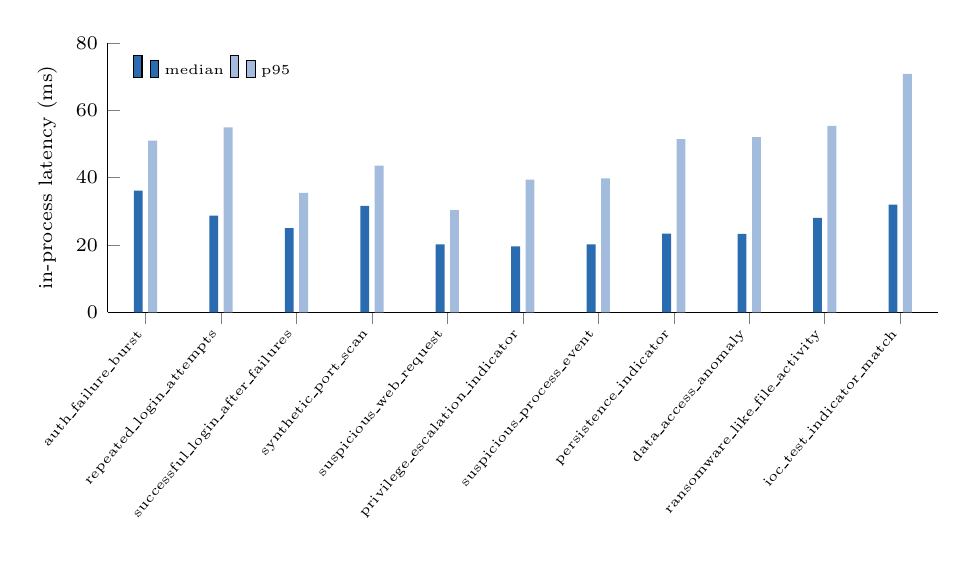
\begin{tikzpicture}
\begin{axis}[
  width=\columnwidth, height=5.0cm, ybar, bar width=3.2pt, ymin=0, ymax=80,
  ylabel={in-process latency (ms)}, ylabel style={font=\scriptsize},
  symbolic x coords={auth\_failure\_burst,repeated\_login\_attempts,successful\_login\_after\_failures,synthetic\_port\_scan,suspicious\_web\_request,privilege\_escalation\_indicator,suspicious\_process\_event,persistence\_indicator,data\_access\_anomaly,ransomware\_like\_file\_activity,ioc\_test\_indicator\_match},
  xtick=data, x tick label style={rotate=50, anchor=east, font=\tiny},
  tick label style={font=\scriptsize}, enlarge x limits=0.05,
  axis x line*=bottom, axis y line*=left,
  legend style={font=\tiny, at={(0.02,0.98)}, anchor=north west, draw=none}, legend columns=2]
\addplot[fill=cdblue, draw=none] coordinates {(auth\_failure\_burst,36.2) (repeated\_login\_attempts,28.7) (successful\_login\_after\_failures,25.0) (synthetic\_port\_scan,31.6) (suspicious\_web\_request,20.2) (privilege\_escalation\_indicator,19.6) (suspicious\_process\_event,20.2) (persistence\_indicator,23.4) (data\_access\_anomaly,23.3) (ransomware\_like\_file\_activity,28.1) (ioc\_test\_indicator\_match,32.0)};
\addplot[fill=clblue, draw=none] coordinates {(auth\_failure\_burst,51.0) (repeated\_login\_attempts,55.0) (successful\_login\_after\_failures,35.5) (synthetic\_port\_scan,43.6) (suspicious\_web\_request,30.4) (privilege\_escalation\_indicator,39.4) (suspicious\_process\_event,39.8) (persistence\_indicator,51.5) (data\_access\_anomaly,52.1) (ransomware\_like\_file\_activity,55.4) (ioc\_test\_indicator\_match,70.9)};
\legend{median, p95}
\end{axis}
\end{tikzpicture}
\caption{In-process scenario latency (median and p95), 20 runs per scenario (E2).}
\label{fig:latency}
\end{figure}

% ---------------- Fig. 7 ----------------
% Values for 400 and 1000 users are from the text. The 100-user curve was read off the
% original chart (approximate) - replace with exact values from your E5 CSV if available.
% 25 users raised no alerts at any p and cannot be drawn on a log axis.
\begin{figure}[t]
\centering
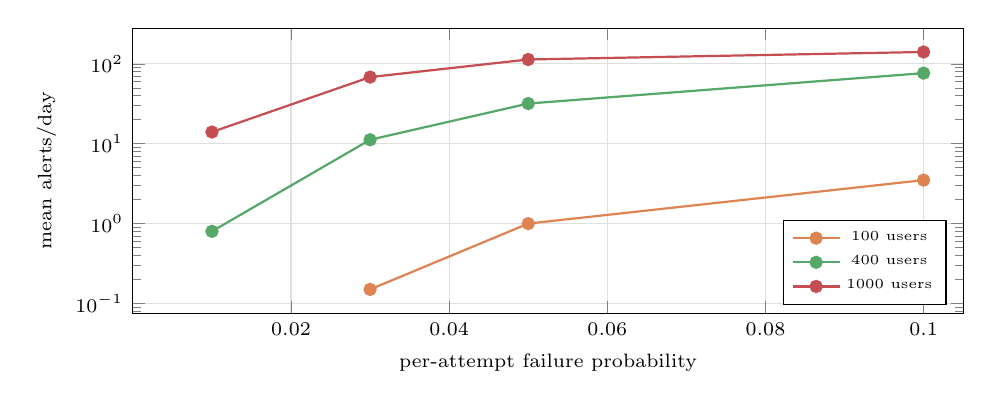
\begin{tikzpicture}
\begin{axis}[
  width=\columnwidth, height=5.2cm, ymode=log, xmin=0, xmax=0.105,
  xlabel={per-attempt failure probability}, ylabel={mean alerts/day},
  label style={font=\scriptsize}, tick label style={font=\scriptsize},
  xtick={0.02,0.04,0.06,0.08,0.10}, grid=major, grid style={gray!25},
  legend style={font=\tiny, at={(0.98,0.03)}, anchor=south east},
  xticklabel style={/pgf/number format/fixed, /pgf/number format/precision=2}]
\addplot[mark=*, thick, color=corange] coordinates {(0.03,0.15) (0.05,1.0) (0.10,3.5)};
\addplot[mark=*, thick, color=cgreen]  coordinates {(0.01,0.8) (0.03,11.2) (0.05,31.8) (0.10,76.4)};
\addplot[mark=*, thick, color=cred]    coordinates {(0.01,14.0) (0.03,68.2) (0.05,113.2) (0.10,140.6)};
\legend{100 users, 400 users, 1000 users}
\end{axis}
\end{tikzpicture}
\caption{Alerts per day from benign users sharing one address (synthetic; 5 seeds per cell). 25 users produced no alerts at any tested $p$.}
\label{fig:noise}
\end{figure}

\subsection{Shared-address noise (E5)}
With $U$ users behind one tackle attacking per day, no alerts emerged at $U=25$ for any failure probability tested ($p\leq 0.10$). At $U=400$, mean alerts per day were 0.8, 11.2, 31.8 and 76.4 for $p=0.01, 0.03, 0.05, 0.10$; at $U=1000$ they were 14.0, 68.2, 113.2 and 140.6 (Fig.~\ref{fig:noise}). Most came from \code{successful\_login\_after\_failures}. This is a attribute of the thresholds under our stated model, not a measured false-positive rate.

\subsection{Throughput and latency (E1)}
Fig.~\ref{fig:tput} is revealing throughput scaling with batch size; for heartbeats the median rose from 34.8 events/s ($B=1$) to 1525.5 ($B=500$), with median request latency 28.7\,ms and 327.8\,ms. Per-request latency at $B=10$ was about 100\,ms, non-monotonic against neighbours; we did not study the cause. At 11,800 stored events, median read latencies were 1.3\,ms (health), 7.4\,ms (events list), 3.7\,ms (alerts list), 29.0\,ms (dashboard summary) and 269.6\,ms (dashboard timeline). Detection runs inside the request, so the figures bundle ingestion and detection. They are outlining one laptop-class VM and are notably not capacity claims.

Table~\ref{tab:tput} and Fig.~\ref{fig:tputlog} show that the batching effect holds across the event types, but its size differs: heartbeats reach about 1526 events/s at $B=500$, authentication successes 1218 and authentication failures with separate sources 940. Failure events cost more per event, because each one also is invoking the authentication-rule queries. The variance is broadly large at small batch sizes (to reveal, heartbeat throughput at $B=1$ ranged from 8 to 66 events/s across 100 requests), so single-event medians should be read with that spread in mind.

The read paths in Fig.~\ref{fig:read} are separating into two groups. Indexed list endpoints and the health check stay in single-digit milliseconds, while the dashboard summary and chiefly the hourly timeline aggregate over the full table, taking 29 and 270\,ms. The timeline is the obvious first target if the stored volume is growing, as any illustration through one more pre-aggregated bucket table.

\begin{table}[t]
\caption{Median ingestion throughput (events/s) and request latency (ms) by event type and batch size, HTTP, SQLite (E1). No alerts were raised in any of these workloads.}
\label{tab:tput}
\centering
\scriptsize
\setlength{\tabcolsep}{3pt}
\begin{tabular}{@{}l r r r r@{}}
\toprule
Event type & $B{=}1$ & $B{=}10$ & $B{=}100$ & $B{=}500$ \\
\midrule
heartbeat (events/s) & 34.8 & 97.3 & 741.5 & 1525.5 \\
\quad latency (ms) & 28.7 & 102.8 & 134.9 & 327.8 \\
auth success (events/s) & 25.7 & 104.8 & 797.5 & 1218.2 \\
\quad latency (ms) & 39.0 & 95.5 & 125.4 & 410.4 \\
auth failure, distinct sources (events/s) & 48.9 & 343.1 & 785.2 & 939.8 \\
\quad latency (ms) & 20.5 & 29.2 & 127.4 & 532.0 \\
\bottomrule
\end{tabular}
\end{table}

% ---------------- Fig. 8 ----------------
\begin{figure}[t]
\centering
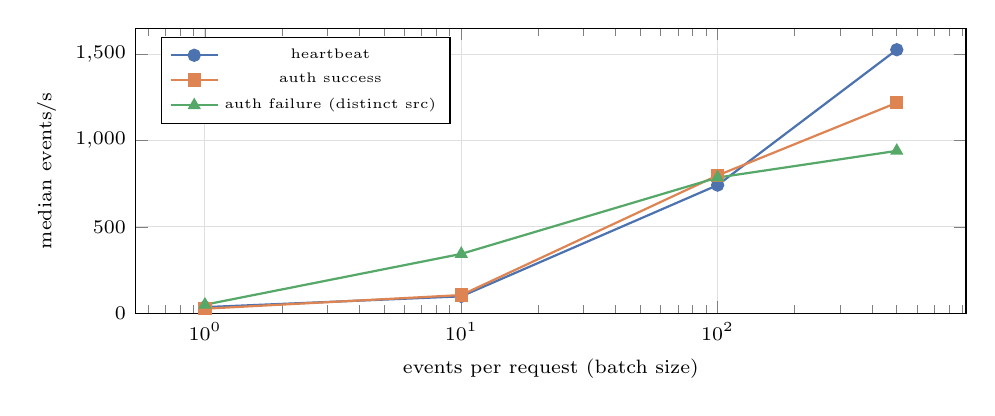
\begin{tikzpicture}
\begin{axis}[
  width=\columnwidth, height=5.2cm, xmode=log, ymin=0, ymax=1650,
  xlabel={events per request (batch size)}, ylabel={median events/s},
  label style={font=\scriptsize}, tick label style={font=\scriptsize},
  grid=major, grid style={gray!25},
  legend style={font=\tiny, at={(0.03,0.97)}, anchor=north west}]
\addplot[mark=*, thick, color=cblue] coordinates {(1,34.8) (10,97.3) (100,741.5) (500,1525.5)};
\addplot[mark=square*, thick, color=corange] coordinates {(1,25.7) (10,104.8) (100,797.5) (500,1218.2)};
\addplot[mark=triangle*, thick, color=cgreen] coordinates {(1,48.9) (10,343.1) (100,785.2) (500,939.8)};
\legend{heartbeat, auth success, auth failure (distinct src)}
\end{axis}
\end{tikzpicture}
\caption{Median ingestion throughput vs.\ batch size over HTTP (SQLite, single process).}
\label{fig:tput}
\end{figure}

% ---------------- Fig. 9 ----------------
\begin{figure}[t]
\centering
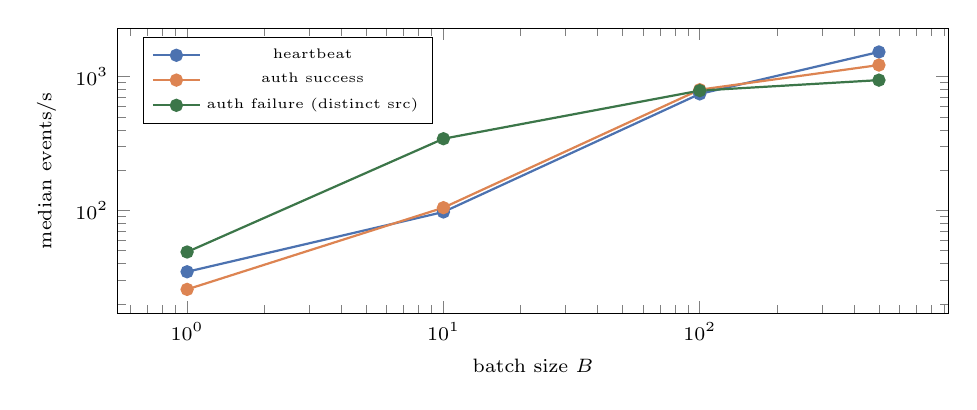
\begin{tikzpicture}
\begin{axis}[
  width=\columnwidth, height=5.2cm, xmode=log, ymode=log,
  xlabel={batch size $B$}, ylabel={median events/s},
  label style={font=\scriptsize}, tick label style={font=\scriptsize},
  legend style={font=\tiny, at={(0.03,0.97)}, anchor=north west}]
\addplot[mark=*, thick, color=cblue] coordinates {(1,34.8) (10,97.3) (100,741.5) (500,1525.5)};
\addplot[mark=*, thick, color=corange] coordinates {(1,25.7) (10,104.8) (100,797.5) (500,1218.2)};
\addplot[mark=*, thick, color=cgreen!70!black] coordinates {(1,48.9) (10,343.1) (100,785.2) (500,939.8)};
\legend{heartbeat, auth success, auth failure (distinct src)}
\end{axis}
\end{tikzpicture}
\caption{Median throughput by event type and batch size (log--log).}
\label{fig:tputlog}
\end{figure}

% ---------------- Fig. 10 ----------------
% Medians are from the text; p95 values were read off the original chart (approximate).
\begin{figure}[t]
\centering
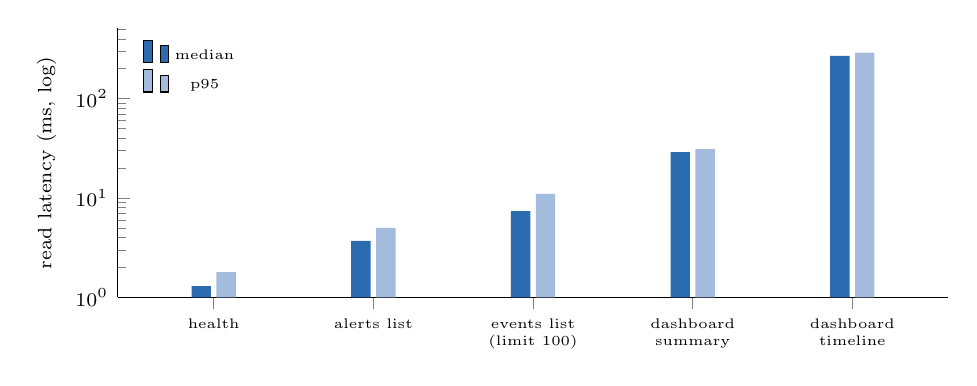
\begin{tikzpicture}
\begin{axis}[
  width=\columnwidth, height=5.0cm, ybar, bar width=7pt, ymode=log, ymin=1, log origin=infty,
  ylabel={read latency (ms, log)}, ylabel style={font=\scriptsize},
  symbolic x coords={health,alerts,events,summary,timeline}, xtick=data,
  xticklabels={health, alerts list, {events list\\(limit 100)}, {dashboard\\summary}, {dashboard\\timeline}},
  x tick label style={font=\tiny, align=center}, tick label style={font=\scriptsize},
  enlarge x limits=0.15, axis x line*=bottom, axis y line*=left,
  legend style={font=\tiny, at={(0.02,0.98)}, anchor=north west, draw=none}]
\addplot[fill=cdblue, draw=none] coordinates {(health,1.3) (alerts,3.7) (events,7.4) (summary,29.0) (timeline,269.6)};
\addplot[fill=clblue, draw=none] coordinates {(health,1.8) (alerts,5.0) (events,11.0) (summary,31.0) (timeline,290.0)};
\legend{median, p95}
\end{axis}
\end{tikzpicture}
\caption{Read-path latency on 11,800 stored events (30 requests each).}
\label{fig:read}
\end{figure}

\subsection{Input sturdiness (E9)}
Of 37 cases, 27 strict expectations were met, namely format and field errors returned 400, wrong payload shapes 422, unauthenticated requests 401 and viewer writes 403; batch writes were atomic, secrets were, in practice, redacted and SQL-injection strings were stored inertly. Six cases caused server failures (a list-valued host, one dict-valued host, a non-numeric port, an oversized port, a dict-valued username and an integer message). The service stayed healthy afterwards. The syntactically invalid tackle 999.1.1.1 was accepted, so no address validation applies. We did not adjust the application; type validation at the schema layer is the obvious solve.

The failure cases in Table~\ref{tab:robust} are sharing one cause, like the nor- A value of the wrong type is accepted by malizer and a later step (a database insert or string operation) fails. Of the 37 cases, 27 met their strict expectation; 10 were exploratory probes without one. Six of these ten caused a server failure, three returned HTTP 500 and three ended with the connection closed without a response, while the other four were accepted and stored. None left the service unhealthy, and the post-test health check passed. Because the failures are reached by an authenticated analyst and not by an anonymous caller, the exposure is bounded, but it is still the most direct improvement available.

\begin{table}[t]
\caption{Robustness cases by class (E9).}
\label{tab:robust}
\centering
\scriptsize
\setlength{\tabcolsep}{3pt}
\begin{tabular}{@{}p{3.4cm} c p{3.0cm}@{}}
\toprule
Class & Cases & Observed outcome \\
\midrule
Unknown format, missing field, bad value & 11 & 400 (as specified) \\
Wrong payload shape, invalid JSON & 4 & 422 \\
Unauthenticated / viewer write & 2 & 401 / 403 \\
Empty batch, batch atomicity & 2 & 400, nothing stored \\
Oversize, nesting, Unicode, injection, valid address & 6 & accepted (201) and stored inertly \\
Secret redaction, post-test health & 2 & as specified \\
Control characters, long string, invalid address & 3 & accepted (201); no strict expectation \\
Wrong field type (list, dict, text/large port, integer) & 7 & 1 accepted, 3 HTTP 500, 3 dropped \\
\bottomrule
\end{tabular}
\end{table}

\subsection{QRI properties (R1)}
On 2000 random inventories, CR equalled QE in every case and also equalled MP, and the default QRI equalled $0.7\,\mathrm{CR}+0.3\,\mathrm{MP}$ exactly. Spearman correlation against the default ranking was 1.0 for all 66 alternative weight vectors, so the weights change magnitudes but not orderings on this generator. Unclassified algorithms are the notable edge: CR and QE count them as non-HIGH, whereas MP treats them as not prepared. Ten unclassified assets yield $\mathrm{CR}=100$, $\mathrm{MP}=0$, $\mathrm{QRI}=70$, while ten RSA-2048 assets yield $\mathrm{QRI}=0$. The CR$-$MP gap grows linearly with the unclassified fraction (Fig.~\ref{fig:gap}). Reference inventories scored 40 (legacy-heavy), 60 (mixed transition) and 100 (PQ-first). Because CR, MP and QE coincide on catalog-only inventories, the index offers no independent information from its three components there. The demonstration inventory (Table~\ref{tab:demoinv}) contains two UNKNOWN algorithms, so this behaviour is not hypothetical.

Tables~\ref{tab:refinv} and~\ref{tab:unclass} make the index behaviour concrete. Over 2000 random inventories the mean QRI was 66.9 (standard deviation 14.2, 95th percentile 87.5). Adding unclassified assets raises the mean index, from 66.8 with none to 70.0 with all assets unclassified, which is the opposite of what a cautious tool should do when it knows less about an inventory. This directly motivates the recommendation to report unclassified assets as their own bucket.

% ---------------- Fig. 11 ----------------
\begin{figure}[t]
\centering
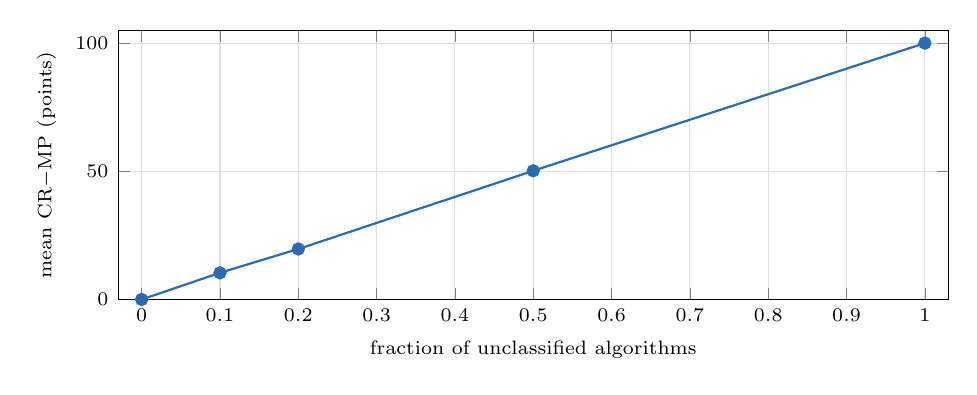
\begin{tikzpicture}
\begin{axis}[
  width=\columnwidth, height=5.0cm, xmin=-0.03, xmax=1.03, ymin=0, ymax=105,
  xlabel={fraction of unclassified algorithms}, ylabel={mean CR$-$MP (points)},
  label style={font=\scriptsize}, tick label style={font=\scriptsize},
  grid=major, grid style={gray!25}]
\addplot[mark=*, thick, color=cdblue] coordinates {(0.0,0.0) (0.1,10.4) (0.2,19.7) (0.5,50.2) (1.0,100.0)};
\end{axis}
\end{tikzpicture}
\caption{Mean CR$-$MP gap vs.\ fraction of unclassified algorithms (R1).}
\label{fig:gap}
\end{figure}

\begin{table}[t]
\caption{Reference inventories and edge cases for the QRI (R1).}
\label{tab:refinv}
\centering
\footnotesize
\setlength{\tabcolsep}{3pt}
\begin{tabular}{@{}p{4.2cm} r r r r@{}}
\toprule
Inventory (10 assets) & CR & MP & QE & QRI \\
\midrule
Legacy-heavy (4 RSA-2048, 2 ECDSA, 2 AES-128, 2 SHA-256) & 40 & 40 & 40 & 40 \\
Mixed (2 RSA-2048, 2 ECDH, 2 hybrid KEM, 2 ML-DSA-65, 2 AES-256) & 60 & 60 & 60 & 60 \\
PQ-first (hybrid and ML-KEM, ML-DSA-65, AES-256) & 100 & 100 & 100 & 100 \\
Ten RSA-2048 assets & 0 & 0 & 0 & 0 \\
Ten unclassified assets & 100 & 0 & 100 & 70 \\
\bottomrule
\end{tabular}
\end{table}

\begin{table}[t]
\caption{Effect of unclassified algorithms on the index (R1; mean over random inventories).}
\label{tab:unclass}
\centering
\footnotesize
\begin{tabular}{@{}c r r@{}}
\toprule
Fraction unclassified & Mean CR$-$MP & Mean QRI \\
\midrule
0.0 & 0.0 & 66.8 \\
0.1 & 10.4 & 67.4 \\
0.2 & 19.7 & 67.4 \\
0.5 & 50.2 & 69.2 \\
1.0 & 100.0 & 70.0 \\
\bottomrule
\end{tabular}
\end{table}

\subsection{Quantum demonstrations (Q1--Q3)}
Ideal Grover runs succeeded with probability 1.0 (80 runs). Under depolarizing noise ($p_2=10p_1$, 20 repetitions of 1024 shots) mean success fell from 1.0000 ($p_1=0$) to 0.9648 at $10^{-3}$, 0.7114 at $10^{-2}$ and 0.2979 at $5\times 10^{-2}$ (Fig.~\ref{fig:grover}). In basis $\{rz, sx, x, cx\}$ the circuit has depth 26. The Shor toy ($N=15$, $a=7$, 8 qubits) recovered $\{3,5\}$ in 50/50 runs at 1024 shots; its depth is 189 in Aer's gate set and 1700 in the restricted basis (888 CX). Under these conditions, all these are revealing one unimportant instance and say nothing about the feasibility of attacks on real keys, for which see~\cite{gidney2021}.

Table~\ref{tab:circuits} places the two circuits side by side. The Shor outcomes are widely close to uniform over the four values that are multiples of $16/r$, as theory projects for $r=4$, and any further chi-square statistic of about 1.3 on three degrees of freedom is uniform with equal probabilities. The jump from the depth of 26 to 1700 for the smallest non-trivial factoring instance reveals, without any claim about real keys, why resource approximations for 2048-bit moduli~\cite{gidney2021} are regularly so large.

% ---------------- Fig. 12 ----------------
% Values at 1e-3, 1e-2 and 5e-2 are from the text; intermediate points were read off the
% original chart (approximate). The p1 = 0 point is drawn at the left edge (3e-5).
\begin{figure}[t]
\centering
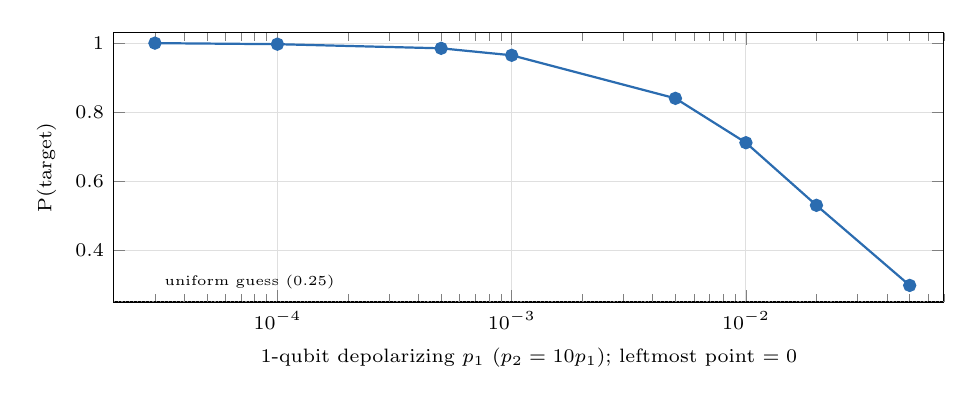
\begin{tikzpicture}
\begin{axis}[
  width=\columnwidth, height=5.0cm, xmode=log, xmin=2e-5, xmax=7e-2, ymin=0.25, ymax=1.03,
  xlabel={1-qubit depolarizing $p_1$ ($p_2=10p_1$); leftmost point $=0$}, ylabel={P(target)},
  label style={font=\scriptsize}, tick label style={font=\scriptsize},
  grid=major, grid style={gray!25}]
\addplot[mark=*, thick, color=cdblue] coordinates {(3e-5,1.0) (1e-4,0.997) (5e-4,0.985) (1e-3,0.9648) (5e-3,0.84) (1e-2,0.7114) (2e-2,0.53) (5e-2,0.2979)};
\draw[densely dotted, gray] (axis cs:2e-5,0.25) -- (axis cs:7e-2,0.25);
\node[font=\tiny, anchor=south west] at (axis cs:3e-5,0.26) {uniform guess (0.25)};
\end{axis}
\end{tikzpicture}
\caption{Grover success vs.\ depolarizing noise.}
\label{fig:grover}
\end{figure}

\begin{table}[t]
\caption{Quantum circuit statistics (Q2, Q3).}
\label{tab:circuits}
\centering
\scriptsize
\setlength{\tabcolsep}{3pt}
\begin{tabular}{@{}l r r@{}}
\toprule
Quantity & Grover (2 qubits) & Shor ($N=15$, $a=7$) \\
\midrule
Logical qubits & 2 & 8 (4 counting, 4 work) \\
Depth, Aer gate set & -- & 189 \\
Depth, basis $\{rz,sx,x,cx\}$ & 26 & 1700 \\
CX gates, basis & 2 & 888 \\
Other gates & 20 rz, 10 sx, 4 x & 1519 rz, 278 sx, 1 x \\
Shor counts of 0, 4, 8, 12 & -- & 1018, 997, 1037, 1044 \\
\bottomrule
\end{tabular}
\end{table}

\subsection{Signing cost (S1)}
ML-DSA-65 signatures are 3309\,B with 1952\,B public keys, against 70\,B (ECDSA P-256, DER) and 384\,B (RSA-3072) signatures. For report-sized payloads the extra time is milliseconds (Table~\ref{tab:signing}).

\begin{table}[t]
\caption{Median sign/verify time in ms (30 repetitions) by payload size.}
\label{tab:signing}
\centering
\scriptsize
\setlength{\tabcolsep}{3pt}
\begin{tabular}{@{}l c c c c@{}}
\toprule
Scheme & 1\,KiB & 100\,KiB & 1\,MiB & 10\,MiB \\
\midrule
ML-DSA-65 & 0.84/0.17 & 0.96/0.40 & 3.31/2.51 & 25.63/25.09 \\
ECDSA-P256 & 0.04/0.09 & 0.11/0.16 & 0.81/0.80 & 7.60/7.57 \\
RSA-3072-PSS & 1.88/0.06 & 1.97/0.12 & 2.66/0.77 & 9.45/7.44 \\
\bottomrule
\end{tabular}
\end{table}

% =====================================================================
\section{Evidence Status and Shortcomings}\label{sec:limits}
% =====================================================================
Documentation and code are disagreeing in places -- the detection-rule document and README list older MITRE mappings or 16 rules (code: 17), one document says 10 situations (code: 11), and 172 backend tests are reported by documents (we gathered 193). We follow the code. The demonstration run of Section~\ref{sec:demo} applied a development-mode instance (SQLite, Vite server), not the Docker/nginx/PostgreSQL deployment, which we did not run. Further shortcomings -- all event data are synthetic; one host; SQLite only; no comparison with another SOC platform; no user study. The 19 cited works are, in practice, journal articles; each was checked against Crossref for metadata and against SCImago (SJR 2025) for quartile, and each individual venue is substantially ranked Q1 as its best quartile. One venue, Sensors, is reliably Q1 in electrical and electronic engineering but Q2 in information systems; a candidate magazine (IEEE Security \& Privacy) was excluded because its Q1 ranking is only in the Law category. Quartiles are, in effect, current rankings, not those at publication, and are commonly listed in \code{references\_verification.csv}.

\subsection{Threats to validity}
\emph{Construct validity.} A case is passing when the declared rule fires, so the validation measures agreement between a generator and a rule written by the same authors. It lays out that the pipeline is, in this setting, wired correctly and that the negative control is sensitive; it does not reveal that the rules detect real opponents. \emph{Internal validity.} Timing was, in essence, taken on a two-core virtual machine whose host load we did not control, which is, in practice, explaining some of the spread (as an illustration the 62.8\,ms standard departure of the threat-intelligence situation against a 32\,ms median). Seeds are fixed and recorded. \emph{External validity.} All events are, in essence, synthetic, the database is SQLite, and there is one host; PostgreSQL, multiple workers, TLS termination and real agents may, in essence, change both throughput and failure modes. \emph{Conclusion validity.} Counts such as 20 repetitions per case tightly bound on a deterministic pipeline but say little about rare faults; the noise experiment E5 is a model with stated factors. \emph{Metric validity.} The QRI is a suggested research metric; its three parts coincide on catalogued inventories, so its apparent richness is partially an artefact of the definition.

\subsection{Testing practice and operations}
Beyond the trials, the store carries its own checks -- 19 backend test files (193 passing tests, of which 167 are statically visible functions, the remainder originating from parametrization) and four root test files with 17 tests covering the agent, the real-server end-to-end flow (enrollment, single-apply token, ingestion to alert, offline buffering, revocation), the demonstration script and the full chain from ingestion to dashboard. One further mutation sanity check, which is disabling the endpoint-state check in the security dependencies, is making the revoked-credential test fail, checking that the tests can fail. Any automated browser script with 31 checks was run against a natively started server in an earlier environment and is not part of the continuous-integration suite. For rollout, the target is Docker Compose with PostgreSQL and an nginx stand-in; this stack, its backup and restore method and remote access were not executed in the build environment (Table~\ref{tab:status}). The login limiter and the live-event stream are per-process, so multi-worker rollout is typically flagged as not realized.

\begin{table}[t]
\caption{Verification status (repository's own report, plus this study).}
\label{tab:status}
\centering
\footnotesize
\begin{tabular}{@{}l p{5.6cm}@{}}
\toprule
Status & Items \\
\midrule
Pass & backend and root tests (re-run); frontend build; Playwright 31/31 (earlier environment, not in CI); ML-DSA-65 signing; demonstration run of Section~\ref{sec:demo} \\
Partial & Windows agent (fixture data only); agent over TLS (end-to-end test ran over plain HTTP in lab mode) \\
Blocked & Docker deployment; LAN/remote access; backup/restore; nginx hybrid TLS \\
Not implemented & multi-worker live stream; PQ server certificate; ML-DSA-signed JWTs; CI browser tests \\
Not claimed & certification; production grade \\
\bottomrule
\end{tabular}
\end{table}

% =====================================================================
\section{Discussion and Future Work}
% =====================================================================
The use is revealing that the detection pipeline behaves as prescribed on its own cases, which is a regression-style statement and not an accuracy claim; the negative control guards against a shallow check (RQ1). Throughput and latency are, in effect, satisfactory for a laboratory deployment, with batching as the primary lever, and the robustness probe spots concrete, fixable weaknesses in input validation (RQ2). The more valuable findings are, in practice, the edges -- shared-address noise, low-and-slow evasion, deduplication of address-less events, input type validation, and the unclassified-algorithm asymmetry in the QRI, which indicates treating unclassified assets as an unambiguous, separate risk bucket (RQ3). Future work is encompassing real or public log datasets, a PostgreSQL/Docker deployment run, concurrency testing, adding catalog entries for legacy algorithms such as 3DES and SHA-1, and a usability study of the interface.

\subsection{Lessons for SOC and readiness tooling}
Four concrete lessons are following from the findings. First a detection check that can't fail is generally worthless, so every positive scenario should, in practice, come with a disabled-rule control, as done here. Second, suppression keys decide what an analyst sees: A diverse key (host, user or event are being needed by address-less events hash) or re-runs and genuine repeats will be hidden. Third, thresholds keyed to tackles should be paired with account- or host-keyed rules to cover distributed and slow attacks, and their noise behind shared addresses should be reviewed against the user population. Fourth, a readiness score should never hide what it could not classify; an definite unclassified count costs one line in the interface and removes the inversion laid out in Table~\ref{tab:unclass}.

% =====================================================================
\section{Conclusion}
% =====================================================================
This article supplied Q-SOC, a prototype that is combining rule-based security monitoring with post-quantum readiness assessment behind a person API and dashboard, and gauged it by measurement rather than description. On the detection side, the pipeline from ingestion through the normalization, rule evaluation, alerting and incident handling behaved as stipulated on all 11 controlled situations (220 of 220 runs), and the negative control, which failed 33 of 33 runs with the rule disabled, showed that the validation check is sensitive to the rule rather than shallow. On the quantum side, the assessment engine classified public-key assets as high exposure and symmetric and hash primitives as lower exposure or review, and the Qiskit demonstrations behaved as anticipated on a simulator, while making clear that they are routinely toy instances and not attacks on real keys.

The measurements also exposed weaknesses that a description would have, in practice, hidden. Viewed through this lens, ingestion is principally dominated by per-request overhead, so batching raised median throughput from 35 to 1526 events per second on one laptop-class VM. Six of 37 malformed inputs caused server errors and one invalid tackle was accepted, so schema-level type and address validation is the most direct enhancement. Address-keyed windows miss low-and-slow and distributed attacks and create noise behind shared addresses. In the readiness index, the default weights do not change rankings, and algorithms the catalog can't classify are frequently counted as not at risk by two parts and as not prepared by a third, which can (to a meaningful extent) inflate or twist the score. Recommend reporting unclassified assets as an is therefored definite category, alongside the index, in any rollout.

For practitioners, the principal lesson is that the two concerns can share infrastructure at low cost, such as the cryptographic inventory, assessment and report signing reuse the same authentication, storage, audit and dashboard as the SIEM layer. For researchers, a reproducible use is offered by the prototype that imports the real backend, so each individual claim here can be re-run. The limits are equally clear. All data are consistently synthetic, the proof comes from one machine and SQLite, no comparison with another SOC platform or user study was made, and the Docker, PostgreSQL, remote-access and post-quantum TLS paths are remaining unverified. From this perspective, next stages are, in practice, check on public or real log data, a full containerized deployment test, concurrency and failure-injection testing, a broader algorithm catalog and a study with analysts. Until then, Q-SOC should be read as a recorded, measured research prototype and not as a validated or production-grade product.

\section*{Acknowledgment}
The authors thank their project guide, Dr.\ Syamasudha Veeragadham, School of Computer Science and Engineering, VIT Vellore. An AI assistant was used to help draft, typeset and check this manuscript; the authors are responsible for its content and should disclose this use as the institution requires.

\section*{Reproducibility}
Scripts, raw results and the build procedure are in the \code{paper/} directory of the repository; the demonstration figures and tables are generated by \code{scripts/make\_demo\_figs.py} from \code{data/demo\_data.json}. See \code{README.md}.

% =====================================================================
\begin{thebibliography}{19}
% =====================================================================
\bibitem{vielberth2020}
M.~Vielberth, F.~B\"ohm, I.~Fichtinger, and G.~Pernul, ``Security operations center: A systematic study and open challenges,'' \emph{IEEE Access}, vol.~8, pp.~227756--227779, 2020.

\bibitem{gonzalez2021}
G.~Gonz\'alez-Granadillo, S.~Gonz\'alez-Zarzosa, and R.~Diaz, ``Security information and event management (SIEM): Analysis, trends, and usage in critical infrastructures,'' \emph{Sensors}, vol.~21, no.~14, p.~4759, 2021.

\bibitem{paxson1999}
V.~Paxson, ``Bro: a system for detecting network intruders in real-time,'' \emph{Computer Networks}, vol.~31, no.~23--24, pp.~2435--2463, 1999.

\bibitem{buczak2016}
A.~L. Buczak and E.~Guven, ``A survey of data mining and machine learning methods for cyber security intrusion detection,'' \emph{IEEE Communications Surveys \& Tutorials}, vol.~18, no.~2, pp.~1153--1176, 2016.

\bibitem{khraisat2019}
A.~Khraisat, I.~Gondal, P.~Vamplew, and J.~Kamruzzaman, ``Survey of intrusion detection systems: techniques, datasets and challenges,'' \emph{Cybersecurity}, vol.~2, no.~1, p.~20, 2019.

\bibitem{tounsi2018}
W.~Tounsi and H.~Rais, ``A survey on technical threat intelligence in the age of sophisticated cyber attacks,'' \emph{Computers \& Security}, vol.~72, pp.~212--233, 2018.

\bibitem{georgiadou2021}
A.~Georgiadou, S.~Mouzakitis, and D.~Askounis, ``Assessing MITRE ATT\&CK risk using a cyber-security culture framework,'' \emph{Sensors}, vol.~21, no.~9, p.~3267, 2021.

\bibitem{shor1997}
P.~W. Shor, ``Polynomial-time algorithms for prime factorization and discrete logarithms on a quantum computer,'' \emph{SIAM Journal on Computing}, vol.~26, no.~5, pp.~1484--1509, 1997.

\bibitem{gidney2021}
C.~Gidney and M.~Eker\aa, ``How to factor 2048 bit RSA integers in 8 hours using 20 million noisy qubits,'' \emph{Quantum}, vol.~5, p.~433, 2021.

\bibitem{preskill2018}
J.~Preskill, ``Quantum computing in the NISQ era and beyond,'' \emph{Quantum}, vol.~2, p.~79, 2018.

\bibitem{bernstein2017}
D.~J. Bernstein and T.~Lange, ``Post-quantum cryptography,'' \emph{Nature}, vol.~549, no.~7671, pp.~188--194, 2017.

\bibitem{nejatollahi2019}
H.~Nejatollahi, N.~Dutt, S.~Ray, F.~Regazzoni, I.~Banerjee, and R.~Cammarota, ``Post-quantum lattice-based cryptography implementations: A survey,'' \emph{ACM Computing Surveys}, vol.~51, no.~6, pp.~1--41, 2019.

\bibitem{joseph2022}
D.~Joseph, R.~Misoczki, M.~Manzano, J.~Tricot, F.~D. Pinuaga, O.~Lacombe, S.~Leichenauer, J.~Hidary, P.~Venables, and R.~Hansen, ``Transitioning organizations to post-quantum cryptography,'' \emph{Nature}, vol.~605, no.~7909, pp.~237--243, 2022.

\bibitem{nather2024}
C.~N\"ather, D.~Herzinger, S.-L. Gazdag, J.-P. Stegh\"ofer, S.~Daum, and D.~Loebenberger, ``Migrating software systems toward post-quantum cryptography---a systematic literature review,'' \emph{IEEE Access}, vol.~12, pp.~132107--132126, 2024.

\bibitem{baseri2026}
Y.~Baseri, A.~Hafid, Y.~Shahsavari, D.~Makrakis, and H.~Khodaiemehr, ``Blockchain security risk assessment in quantum era, migration strategies, and proactive defense,'' \emph{IEEE Communications Surveys \& Tutorials}, vol.~28, pp.~2925--2964, 2026.

\bibitem{gisin2002}
N.~Gisin, G.~Ribordy, W.~Tittel, and H.~Zbinden, ``Quantum cryptography,'' \emph{Reviews of Modern Physics}, vol.~74, no.~1, pp.~145--195, 2002.

\bibitem{pirandola2020}
S.~Pirandola, U.~L. Andersen, L.~Banchi, M.~Berta, D.~Bunandar, R.~Colbeck, D.~Englund, T.~Gehring, C.~Lupo, C.~Ottaviani, J.~L. Pereira, M.~Razavi, J.~S. Shaari, M.~Tomamichel, V.~C. Usenko, G.~Vallone, P.~Villoresi, and P.~Wallden, ``Advances in quantum cryptography,'' \emph{Advances in Optics and Photonics}, vol.~12, no.~4, p.~1012, 2020.

\bibitem{tehrani2024}
M.~G. Tehrani, E.~Sultanow, W.~J. Buchanan, M.~Amir, A.~Jeschke, M.~Houmani, R.~Chow, and M.~Lemoudden, ``Stabilized quantum-enhanced SIEM architecture and speed-up through Hoeffding tree algorithms enable quantum cybersecurity analytics in botnet detection,'' \emph{Scientific Reports}, vol.~14, no.~1, p.~1732, 2024.

\bibitem{ring2019}
M.~Ring, S.~Wunderlich, D.~Scheuring, D.~Landes, and A.~Hotho, ``A survey of network-based intrusion detection data sets,'' \emph{Computers \& Security}, vol.~86, pp.~147--167, 2019.

\end{thebibliography}

\end{document}
